\documentclass[12pt,a4paper]{article}

% Packages
\usepackage[utf8]{inputenc}
\usepackage[vietnamese]{babel}
\usepackage[margin=2.5cm]{geometry}
\usepackage{graphicx}
\usepackage{booktabs}
\usepackage{longtable}
\usepackage{array}
\usepackage{multirow}
\usepackage{amsmath}
\usepackage{textcomp}
\usepackage{siunitx}
\usepackage{hyperref}
\usepackage{xcolor}
\usepackage{listings}
\usepackage{fancyhdr}
\usepackage{titlesec}
\usepackage{float}

% Custom commands for special characters
\newcommand{\ugm}{$\mu$g/m$^3$}
\newcommand{\degreec}{$^\circ$C}
\newcommand{\ozone}{O$_3$}
\newcommand{\cotwo}{CO$_2$}
\newcommand{\notwo}{NO$_2$}
\newcommand{\sotwo}{SO$_2$}
\newcommand{\pmtwofive}{PM$_{2.5}$}
\newcommand{\pmten}{PM$_{10}$}

% Formatting
\hypersetup{
    colorlinks=true,
    linkcolor=blue,
    filecolor=magenta,      
    urlcolor=cyan,
}

\setlength{\headheight}{15pt}
\pagestyle{fancy}
\fancyhf{}
\fancyhead[L]{Nhom AIT2006-2-3.4}
\fancyhead[R]{Phan tich Thoi tiet va CL Khong khi}
\fancyfoot[C]{\thepage}

% Title page
\title{
    \vspace{-2cm}
    \textbf{\LARGE BÁO CÁO KỸ THUẬT}\\
    \vspace{0.5cm}
    \textbf{\Large PHÂN TÍCH THỜI TIẾT VÀ CHẤT LƯỢNG KHÔNG KHÍ\\
    TP HỒ CHÍ MINH NĂM 2024}\\
    \vspace{0.5cm}
    \large Môn: Lập trình xử lý dữ liệu
}

\author{
    \textbf{Nhóm: AIT2006-2-3.4}\\
    \vspace{0.3cm}
    \begin{tabular}{ll}
        Tạ Duy Khánh & 24022364 \\
        Nguyễn Đức Vũ Bảo & 24022264 \\
        Đỗ Mạnh Quân & 24022432 \\
    \end{tabular}
}

\date{
    Năm dữ liệu: 2024\\
    Ngày nộp: 19/12/2025\\
    \vspace{0.3cm}
    \small Commit Hash: \texttt{077aa6e244f28f0799fe44e271ba16c4bf332e91}
}

\begin{document}

\maketitle
\thispagestyle{empty}
\newpage

\tableofcontents
\newpage

\section{Giới thiệu và Tổng quan dữ liệu}

\subsection{Mục tiêu dự án}
Dự án này nhằm xử lý, phân tích và dự báo dữ liệu thời tiết và chất lượng không khí cho Thành phố Hồ Chí Minh trong năm 2024. Mục tiêu cụ thể bao gồm:
\begin{itemize}
    \item Làm sạch và chuẩn hóa dữ liệu thời tiết và chất lượng không khí
    \item Tổng hợp thống kê theo nhiều khung thời gian (ngày, tuần, tháng)
    \item Phân tích xu hướng và mối quan hệ giữa các biến
    \item Dự báo nồng độ \pmtwofive{} cho ngày tiếp theo (tính năng nâng cao)
    \item Phân cụm các điều kiện môi trường theo đặc điểm thời tiết
    \item Phát hiện các ngày bất thường về chất lượng không khí
\end{itemize}

\subsection{Nguồn dữ liệu}

\subsubsection{Dữ liệu thời tiết}
\begin{itemize}
    \item \textbf{Nguồn:} Meteostat (\url{https://meteostat.net})
    \item \textbf{File:} \texttt{meteostat\_weather\_data.csv}
    \item \textbf{Phạm vi:} 1/1/2024 - 31/12/2024 (366 ngày)
    \item \textbf{Vị trí:} TP. Hồ Chí Minh (10.823\degreec{}N, 106.6296\degreec{}E)
    \item \textbf{Biến số:} Nhiệt độ, lượng mưa, tốc độ gió, hướng gió, áp suất khí quyển
\end{itemize}

\subsubsection{Dữ liệu chất lượng không khí}
\begin{itemize}
    \item \textbf{Nguồn:} Open-Meteo Air Quality API (\url{https://open-meteo.com})
    \item \textbf{File gốc:} \texttt{open-meteo-hourly-AQ.csv} (dữ liệu theo giờ)
    \item \textbf{File đã xử lý:} \texttt{open-meteo-daily-AQ.csv} (tổng hợp theo ngày)
    \item \textbf{Phạm vi:} 1/1/2024 - 31/12/2024 (366 ngày)
    \item \textbf{Vị trí:} Cùng tọa độ với dữ liệu thời tiết
    \item \textbf{Biến số:} \pmtwofive{}, \pmten{}, CO, \notwo{}, \sotwo{}, \ozone{}, UV Index, Bụi Alder/Birch
\end{itemize}

\subsection{Đặc điểm chính của dữ liệu}

Bảng \ref{tab:data-overview} tổng hợp các đặc điểm chính của tập dữ liệu sau khi làm sạch và tổng hợp:

\begin{table}[H]
\centering
\caption{Tổng quan dữ liệu năm 2024}
\label{tab:data-overview}
\begin{tabular}{ll}
\toprule
\textbf{Đặc điểm} & \textbf{Giá trị} \\
\midrule
Vị trí & TP. Hồ Chí Minh \\
Tọa độ & 10.823\degreec{}N, 106.6296\degreec{}E \\
Năm & 2024 \\
\midrule
Tổng số ngày dữ liệu gốc & 366 ngày \\
Số ngày sau QA (clean) & 366 ngày \\
Tỷ lệ dữ liệu clean & 100.00\% \\
Số tuần & 53 tuần \\
Số tháng & 12 tháng \\
\midrule
Nhiệt độ trung bình năm & 29.10 \degreec{} \\
Tổng lượng mưa năm & 1804.40 mm \\
Số ngày mưa trong năm & 179 ngày \\
\midrule
\pmtwofive{} trung bình năm & 22.67 \ugm{} \\
\pmten{} trung bình năm & 32.32 \ugm{} \\
Số ngày \pmtwofive{} vượt ngưỡng & 132 ngày (36.1\%) \\
Số ngày \pmten{} vượt ngưỡng & 55 ngày (15.0\%) \\
UV Index trung bình năm & 8.83 \\
\bottomrule
\end{tabular}
\end{table}

\section{Làm sạch và Chuẩn hoá dữ liệu}

\subsection{Quy tắc Quality Assurance (QA)}

Dữ liệu được kiểm tra và làm sạch theo các quy tắc sau:

\subsubsection{Dữ liệu thời tiết}
Các vấn đề được phát hiện và xử lý trong dữ liệu thời tiết:

\begin{table}[H]
\centering
\caption{Tóm tắt QA - Dữ liệu thời tiết}
\label{tab:qa-weather}
\begin{tabular}{p{4cm}ccp{6cm}}
\toprule
\textbf{Quy tắc} & \textbf{Số lỗi} & \textbf{Tỷ lệ} & \textbf{Hành động} \\
\midrule
Missing precipitation & 12 & 3.28\% & Gắn cờ \texttt{is\_missing}, giữ nguyên NaN \\
Missing wind direction & 366 & 100\% & Gắn cờ \texttt{is\_missing}, giữ nguyên NaN \\
\bottomrule
\end{tabular}
\end{table}

\textbf{Lưu ý:} Hướng gió thiếu hoàn toàn (100\%) do nguồn dữ liệu không cung cấp. Biến này không được sử dụng trong các phân tích tiếp theo.

\subsubsection{Dữ liệu chất lượng không khí}

\begin{table}[H]
\centering
\caption{Tóm tắt QA - Dữ liệu chất lượng không khí}
\label{tab:qa-airquality}
\begin{tabular}{p{4cm}ccp{6cm}}
\toprule
\textbf{Quy tắc} & \textbf{Số lỗi} & \textbf{Tỷ lệ} & \textbf{Hành động} \\
\midrule
Missing \cotwo{} & 299 & 81.69\% & Gắn cờ \texttt{is\_missing}, giữ nguyên NaN \\
\bottomrule
\end{tabular}
\end{table}

\textbf{Chiến lược xử lý:}
\begin{itemize}
    \item Giữ nguyên giá trị thiếu (NaN) thay vì imputation để tránh tạo bias
    \item Gắn cờ \texttt{is\_missing} cho mỗi biến để tracking
    \item Loại bỏ biến \cotwo{} khỏi các phân tích do tỷ lệ thiếu quá cao
    \item Sử dụng các biến còn lại với độ đầy đủ dữ liệu $>$ 95\%
\end{itemize}

\subsection{Chuẩn hoá dữ liệu}

\subsubsection{Chuẩn hoá thời gian}
\begin{itemize}
    \item Chuyển đổi tất cả timestamps sang định dạng \texttt{YYYY-MM-DD}
    \item Đồng bộ múi giờ UTC cho cả hai nguồn dữ liệu
    \item Tổng hợp dữ liệu hourly thành daily bằng hàm aggregation phù hợp:
    \begin{itemize}
        \item Nhiệt độ, chất lượng không khí: \textbf{trung bình} (mean)
        \item Lượng mưa: \textbf{tổng} (sum)
        \item UV Index: \textbf{giá trị lớn nhất} (max)
    \end{itemize}
\end{itemize}

\subsubsection{Kết hợp dữ liệu (Merge)}

\begin{table}[H]
\centering
\caption{Thống kê quá trình merge dữ liệu}
\label{tab:merge-summary}
\begin{tabular}{lr}
\toprule
\textbf{Chỉ số} & \textbf{Giá trị} \\
\midrule
Records thời tiết (input) & 366 \\
Records chất lượng không khí (input) & 366 \\
Records sau merge (output) & 366 \\
Records bị mất & 0 \\
Tỷ lệ thành công & 100.00\% \\
\midrule
Phương pháp merge & INNER JOIN \\
Khung thời gian & 01/01/2024 - 31/12/2024 \\
Tổng số ngày & 366 ngày \\
\midrule
Số biến thời tiết & 5 \\
Số biến chất lượng không khí & 6 \\
Tổng biến dữ liệu & 11 \\
Tổng cột (bao gồm flags) & 38 \\
\midrule
Records có vấn đề chất lượng & 366 \\
Records không có vấn đề & 0 \\
Độ đầy đủ dữ liệu tổng thể & 83.18\% \\
\bottomrule
\end{tabular}
\end{table}

\section{Tổng hợp và Thống kê}

\subsection{Định nghĩa các chỉ số}

\subsubsection{Air Quality Index (AQI)}
AQI được tính dựa trên nồng độ \pmtwofive{} theo tiêu chuẩn US EPA:

\begin{equation}
\text{AQI} = \frac{I_{high} - I_{low}}{C_{high} - C_{low}} \times (C - C_{low}) + I_{low}
\end{equation}

Trong đó:
\begin{itemize}
    \item $C$: Nồng độ \pmtwofive{} đo được (\ugm{})
    \item $C_{low}$, $C_{high}$: Ngưỡng nồng độ tương ứng với category
    \item $I_{low}$, $I_{high}$: Giá trị AQI tương ứng với category
\end{itemize}

\textbf{Phân loại AQI:}
\begin{itemize}
    \item 0-50: Tốt (Good)
    \item 51-100: Trung bình (Moderate)
    \item 101-150: Không tốt cho nhóm nhạy cảm (Unhealthy for Sensitive Groups)
    \item 151-200: Không tốt (Unhealthy)
    \item 201-300: Rất không tốt (Very Unhealthy)
    \item 301+: Nguy hại (Hazardous)
\end{itemize}

\subsubsection{Normalized Index}
Index chuẩn hóa được tính cho từng biến:

\begin{equation}
\text{Normalized Index} = \frac{X - X_{min}}{X_{max} - X_{min}} \times 100
\end{equation}

Trong đó:
\begin{itemize}
    \item $X$: Giá trị hiện tại
    \item $X_{min}$, $X_{max}$: Giá trị min, max trong cả năm
\end{itemize}

\subsection{Thống kê mô tả}

Dữ liệu được tổng hợp theo 3 khung thời gian:
\begin{itemize}
    \item \textbf{Daily:} Dữ liệu hàng ngày (366 records)
    \item \textbf{Weekly:} Tổng hợp theo tuần (53 records)
    \item \textbf{Monthly:} Tổng hợp theo tháng (12 records)
\end{itemize}

\subsubsection{Thống kê nhiệt độ}

\begin{table}[H]
\centering
\caption{Thống kê nhiệt độ năm 2024}
\label{tab:temp-stats}
\begin{tabular}{lc}
\toprule
\textbf{Chỉ số} & \textbf{Giá trị (\degreec{})} \\
\midrule
Mean (Trung bình) & 29.10 \\
Median (Trung vị) & 29.15 \\
Std (Độ lệch chuẩn) & 1.42 \\
Min (Nhỏ nhất) & 24.85 \\
25th percentile & 28.10 \\
50th percentile (Median) & 29.15 \\
75th percentile & 30.08 \\
Max (Lớn nhất) & 32.40 \\
\bottomrule
\end{tabular}
\end{table}

\subsubsection{Thống kê PM2.5}

\begin{table}[H]
\centering
\caption{Thống kê PM2.5 năm 2024}
\label{tab:pm25-stats}
\begin{tabular}{lc}
\toprule
\textbf{Chỉ số} & \textbf{Giá trị (\ugm{})} \\
\midrule
Mean (Trung bình) & 22.67 \\
Median (Trung vị) & 20.50 \\
Std (Độ lệch chuẩn) & 9.86 \\
Min (Nhỏ nhất) & 6.87 \\
25th percentile & 15.71 \\
50th percentile (Median) & 20.50 \\
75th percentile & 28.04 \\
Max (Lớn nhất) & 56.92 \\
\midrule
Số ngày vượt ngưỡng WHO (15 \ugm{}) & 234 (63.9\%) \\
Số ngày vượt ngưỡng US EPA (35 \ugm{}) & 132 (36.1\%) \\
\bottomrule
\end{tabular}
\end{table}

\section{Trực quan hoá}

Các hình ảnh trực quan hóa được tạo ra để phân tích xu hướng và mối quan hệ giữa các biến. Tất cả các biểu đồ được lưu trong thư mục \texttt{figures/}.

\subsection{Chuỗi thời gian tổng hợp (Meteogram)}

\begin{figure}[H]
\centering
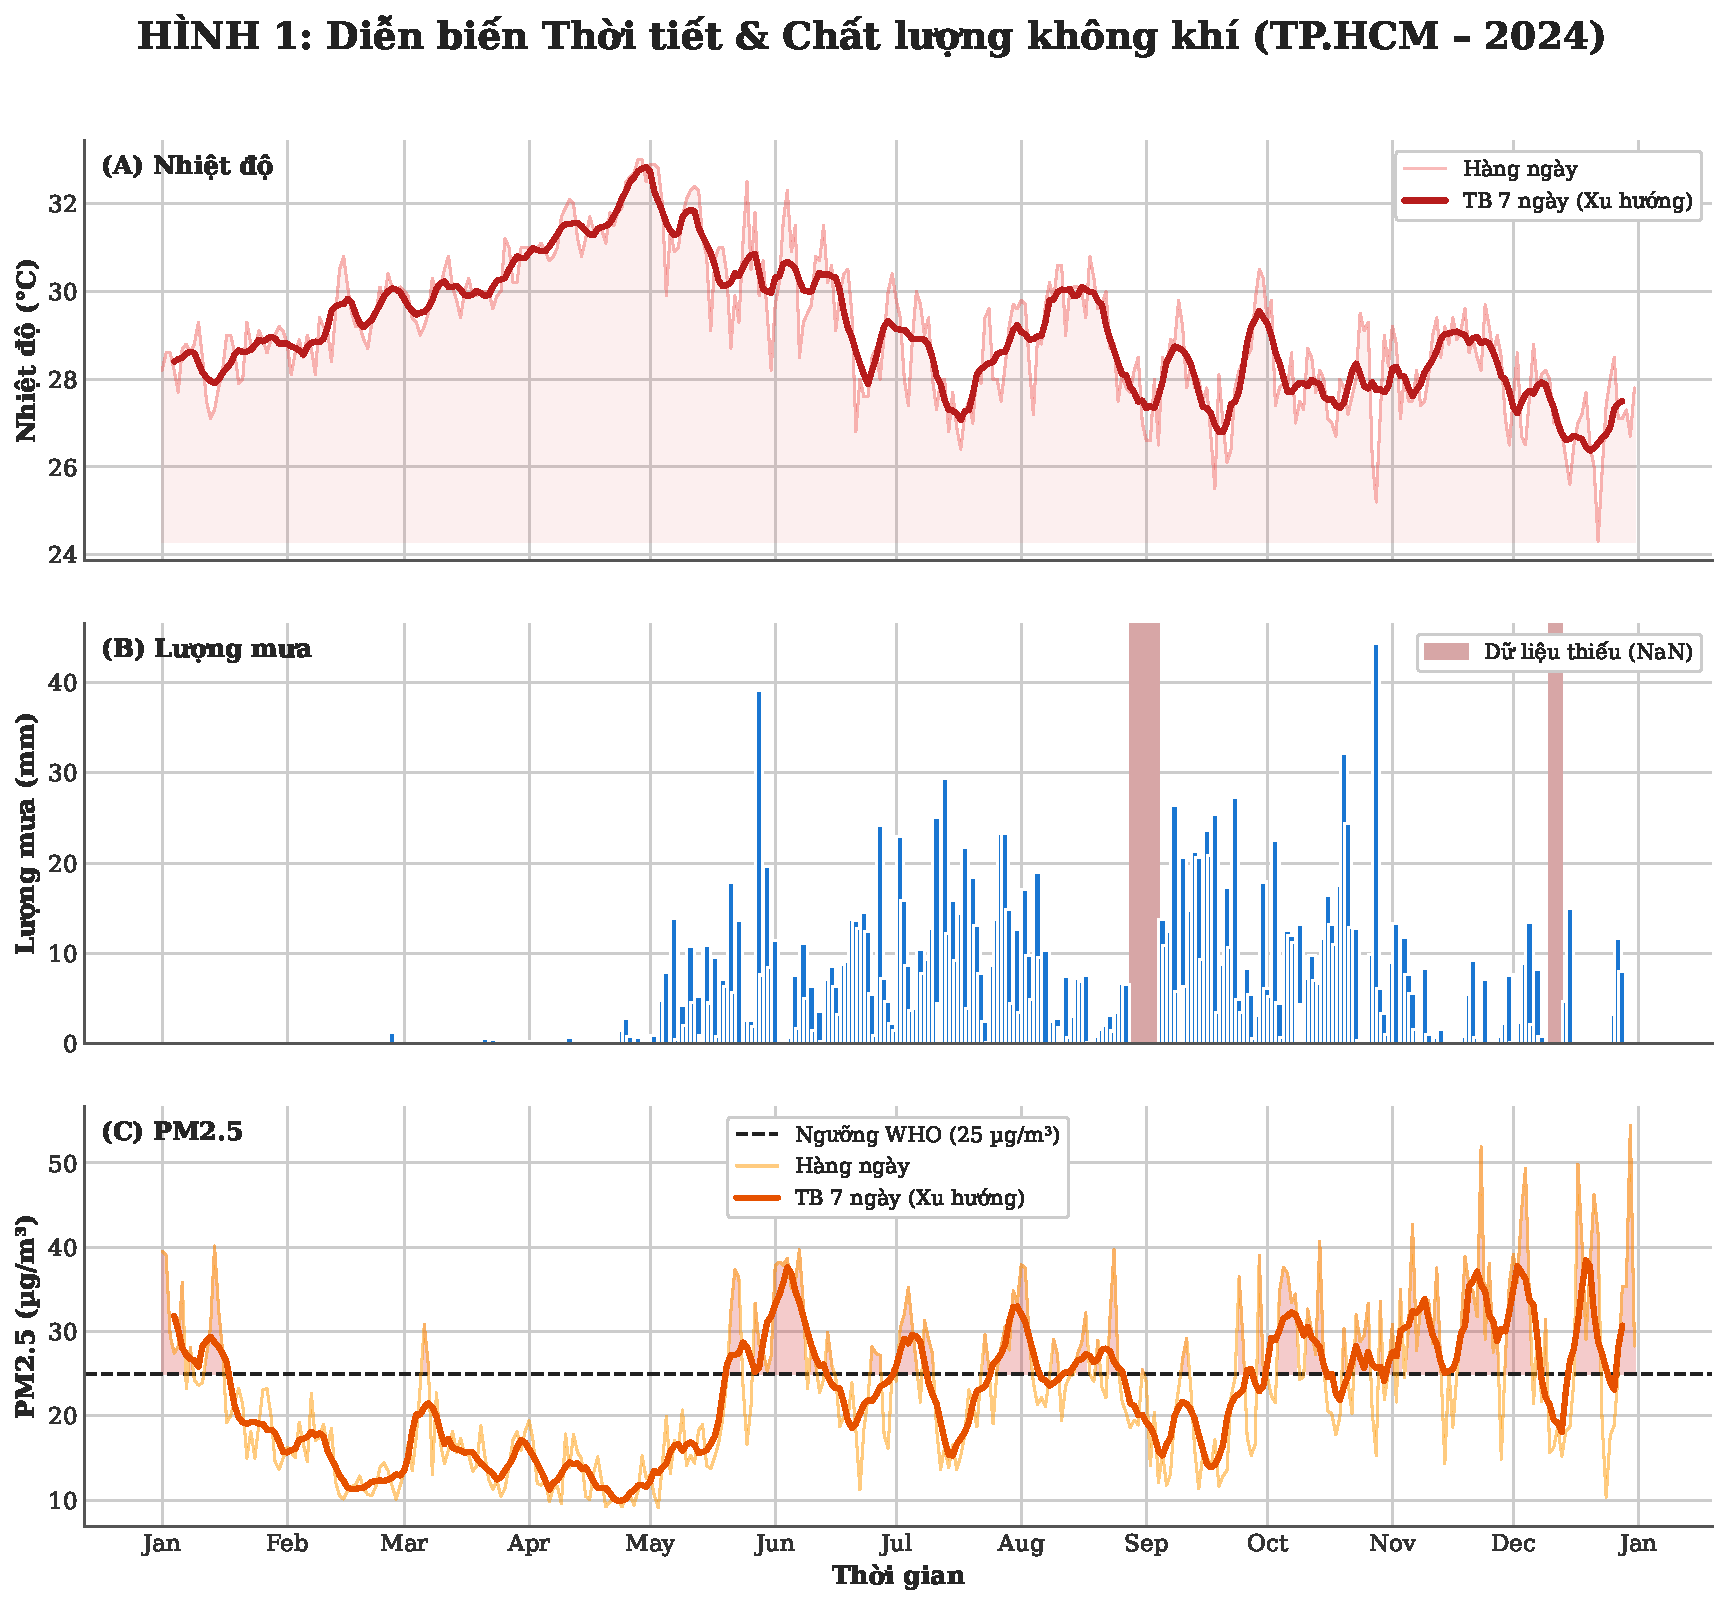
\includegraphics[width=0.95\textwidth]{../figures/01_time_series.pdf}
\caption{Meteogram hiển thị xu hướng đồng thời của nhiệt độ, lượng mưa, \pmtwofive{}, và UV Index năm 2024.}
\label{fig:meteogram}
\end{figure}

\textbf{Nhận xét:}
\begin{itemize}
    \item Meteogram cho phép quan sát mối quan hệ giữa các biến theo thời gian
    \item Nhiệt độ biến động nhẹ quanh 29\degreec{} với đỉnh vào tháng 4-5
    \item Lượng mưa tập trung vào mùa mưa (tháng 5-10)
    \item \pmtwofive{} có xu hướng ngược với lượng mưa
\end{itemize}

\subsection{UV Index theo thời gian}

\begin{figure}[H]
\centering
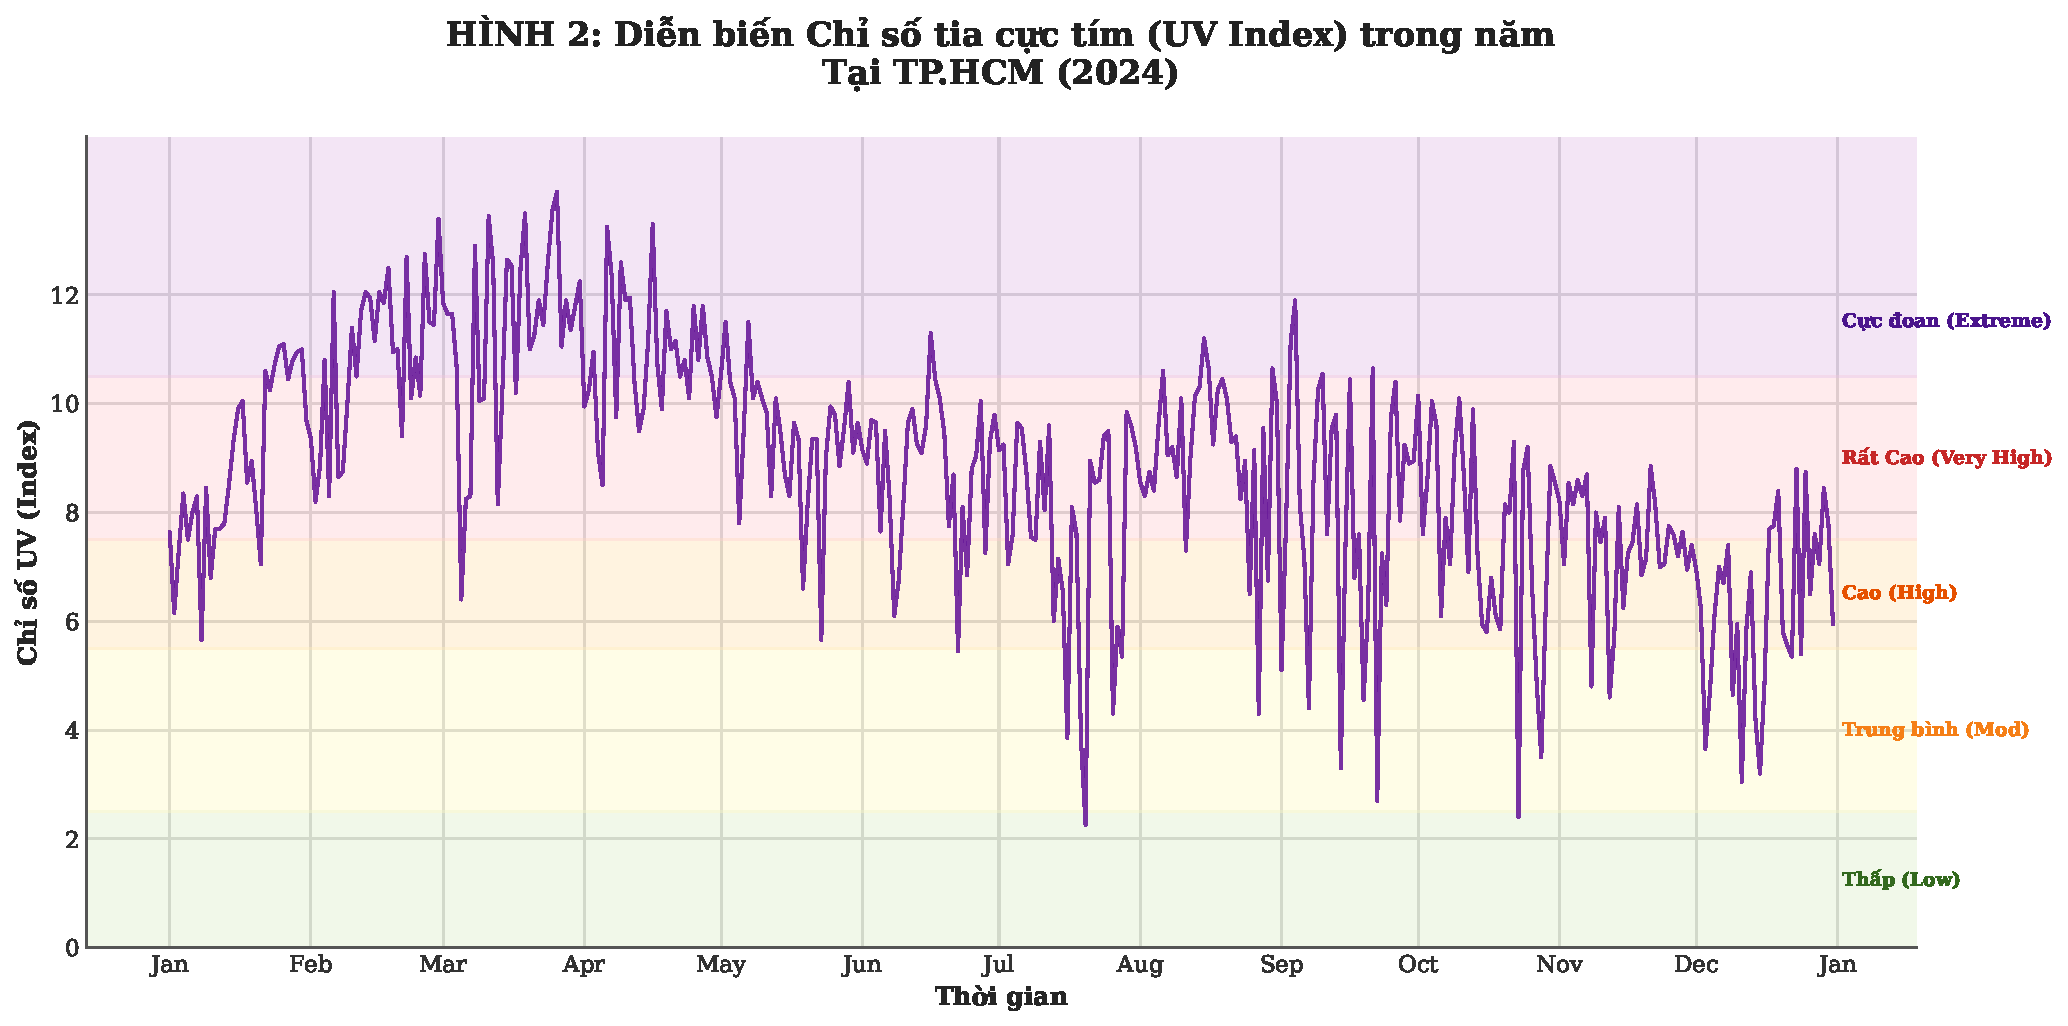
\includegraphics[width=0.95\textwidth]{../figures/02_uv_index.pdf}
\caption{Biến động UV Index năm 2024 với phân loại mức độ nguy hiểm.}
\label{fig:uv-index}
\end{figure}

\textbf{Nhận xét:}
\begin{itemize}
    \item UV Index dao động trong khoảng 5-12, phần lớn ở mức High đến Very High
    \item Mức cao nhất tập trung vào tháng 4-5 (mùa khô)
    \item Giảm nhẹ trong mùa mưa do mây che nhiều
\end{itemize}

\subsection{Phân bố PM2.5}

\begin{figure}[H]
\centering
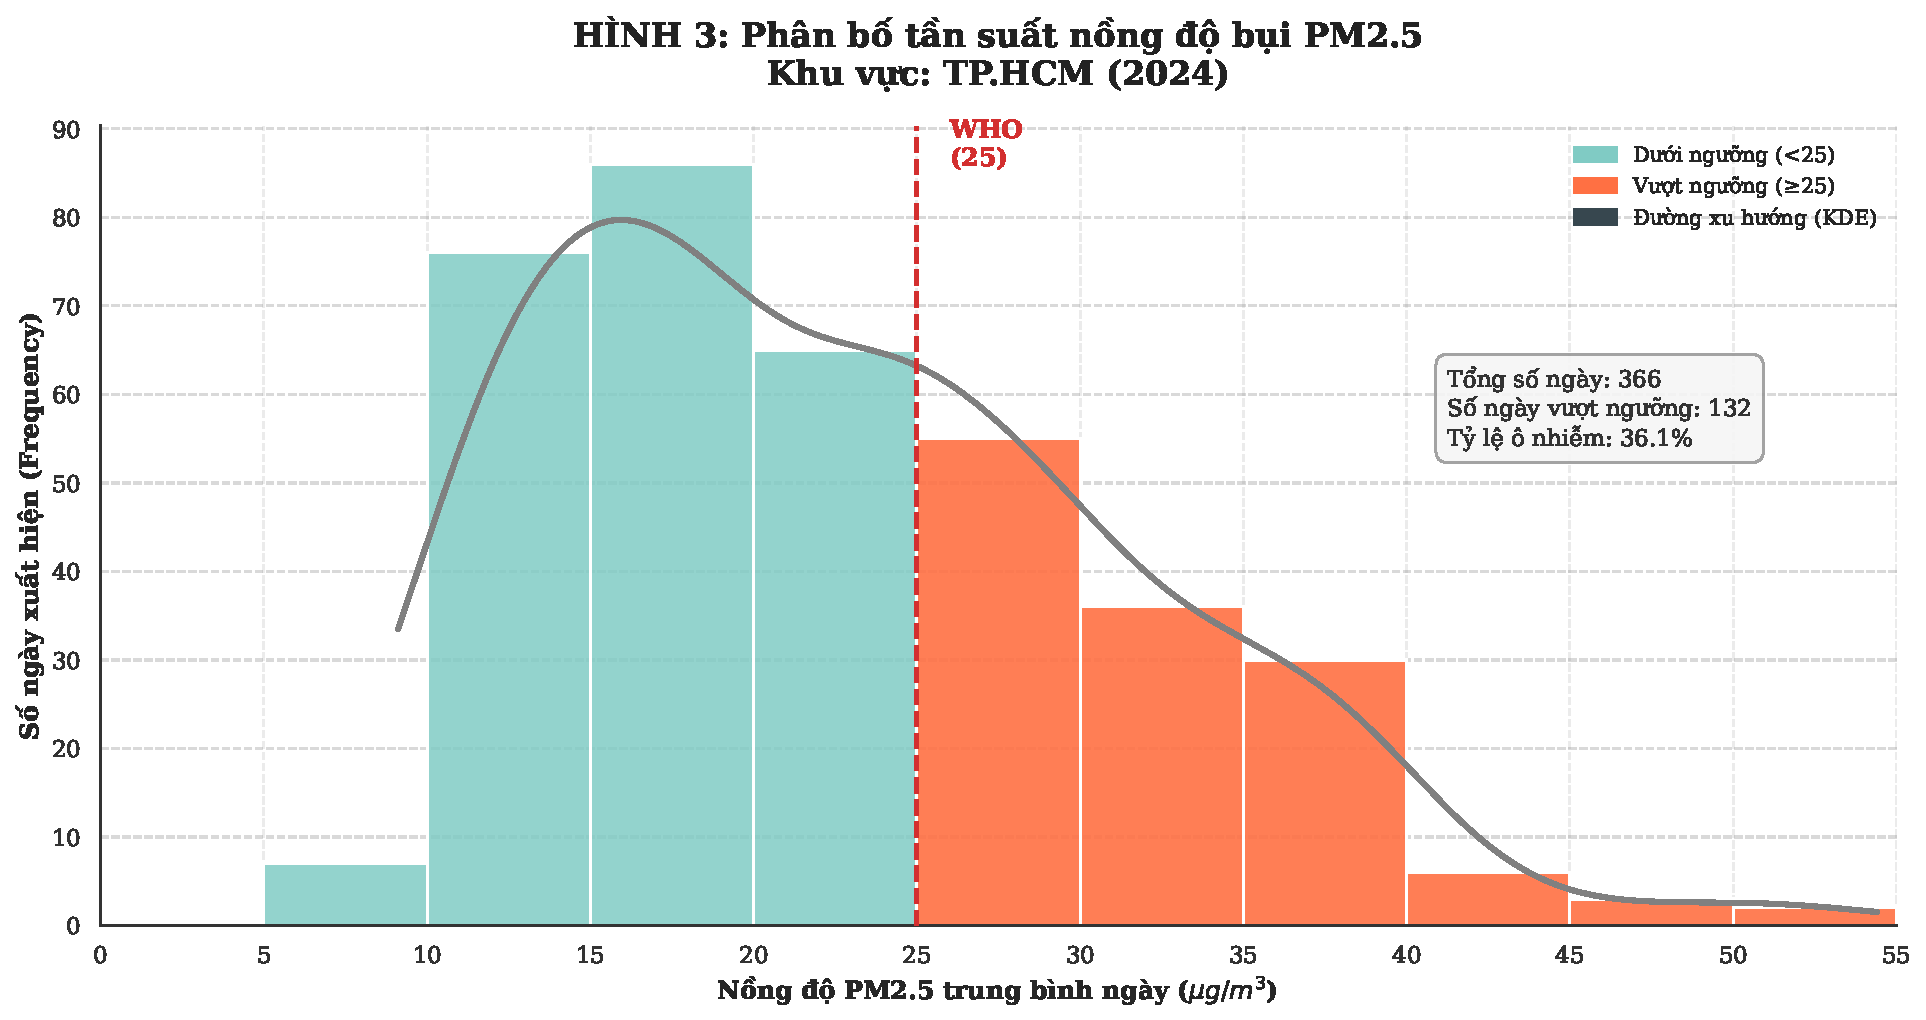
\includegraphics[width=0.95\textwidth]{../figures/03_Pm25_distribution.pdf}
\caption{Phân bố nồng độ \pmtwofive{} năm 2024 với histogram và density plot.}
\label{fig:pm25-distribution}
\end{figure}

\textbf{Nhận xét:}
\begin{itemize}
    \item Phân bố lệch phải (right-skewed) với đuôi dài
    \item Phần lớn giá trị tập trung trong khoảng 15-30 \ugm{}
    \item Có một số giá trị outliers vượt quá 50 \ugm{}
\end{itemize}

\subsection{Xu hướng theo tháng}

\begin{figure}[H]
\centering
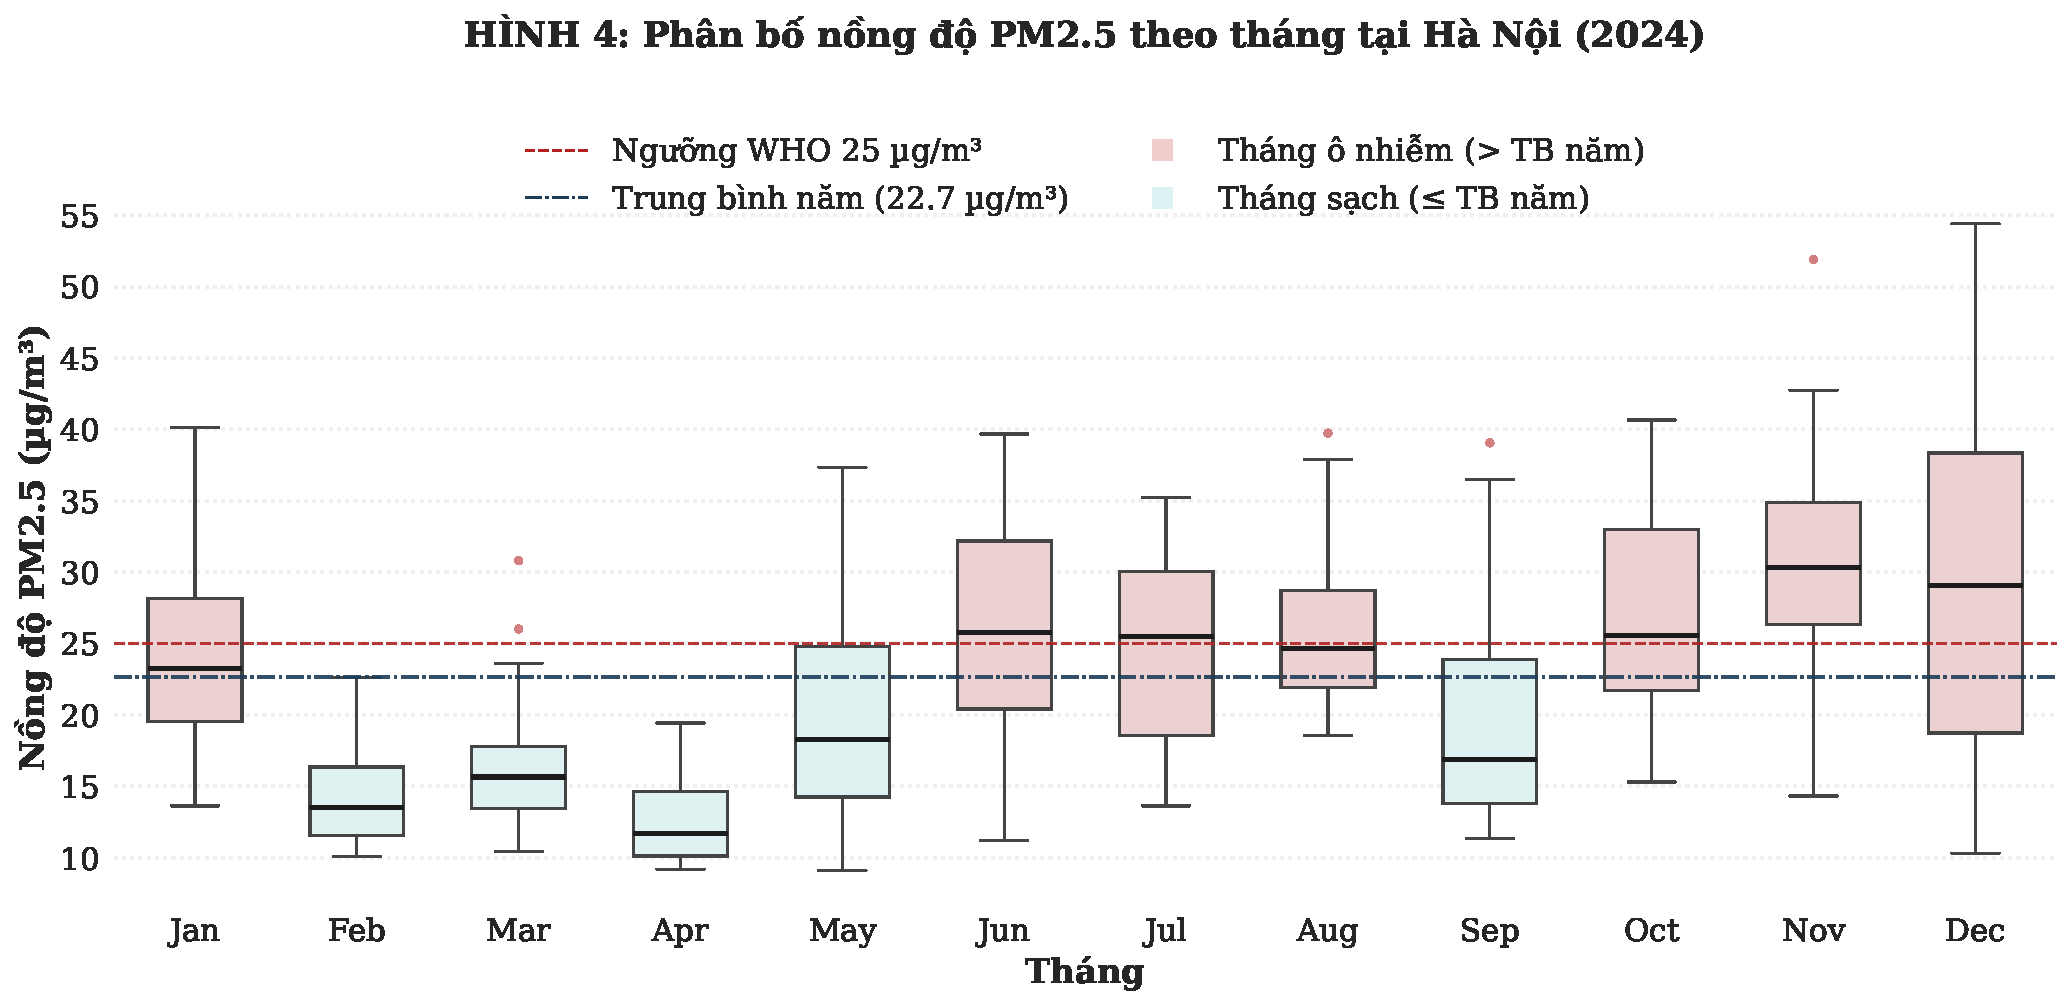
\includegraphics[width=0.95\textwidth]{../figures/04_monthly_boxplot.pdf}
\caption{Boxplot \pmtwofive{} theo từng tháng năm 2024, cho thấy xu hướng theo mùa rõ rệt.}
\label{fig:monthly-boxplot}
\end{figure}

\textbf{Nhận xét:}
\begin{itemize}
    \item Tháng 12, 1, 2, 3 có nồng độ \pmtwofive{} cao nhất (mùa khô)
    \item Tháng 6, 7, 8 có nồng độ thấp nhất (mùa mưa)
    \item Tháng 11-12 có biến động lớn nhất (boxplot dài)
\end{itemize}

\subsection{Ma trận tương quan}

\begin{figure}[H]
\centering
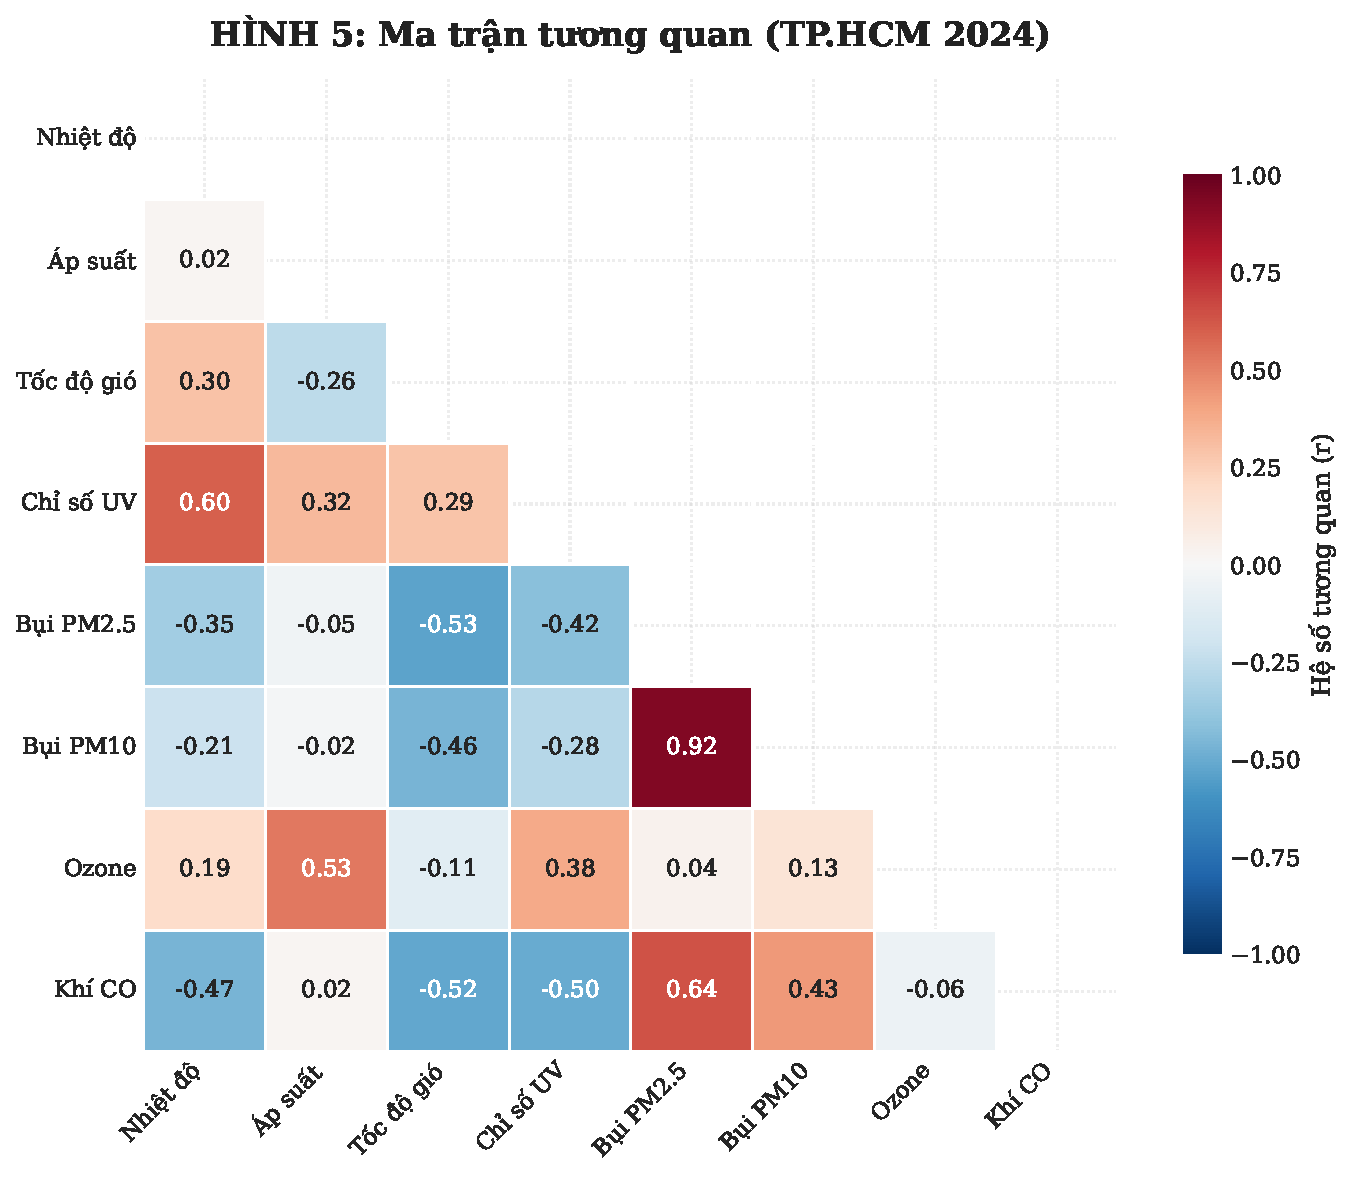
\includegraphics[width=0.95\textwidth]{../figures/05_correlation_matrix.pdf}
\caption{Ma trận tương quan giữa các biến thời tiết và chất lượng không khí.}
\label{fig:correlation-matrix}
\end{figure}

\textbf{Mối tương quan chính:}
\begin{itemize}
    \item \pmtwofive{} và \pmten{}: tương quan dương mạnh (0.85+)
    \item \pmtwofive{} và lượng mưa: tương quan âm (-0.4 đến -0.5)
    \item Nhiệt độ và UV Index: tương quan dương
    \item Lượng mưa và \ozone{}: tương quan âm
\end{itemize}

\subsection{Mối quan hệ gió và PM2.5}

\begin{figure}[H]
\centering
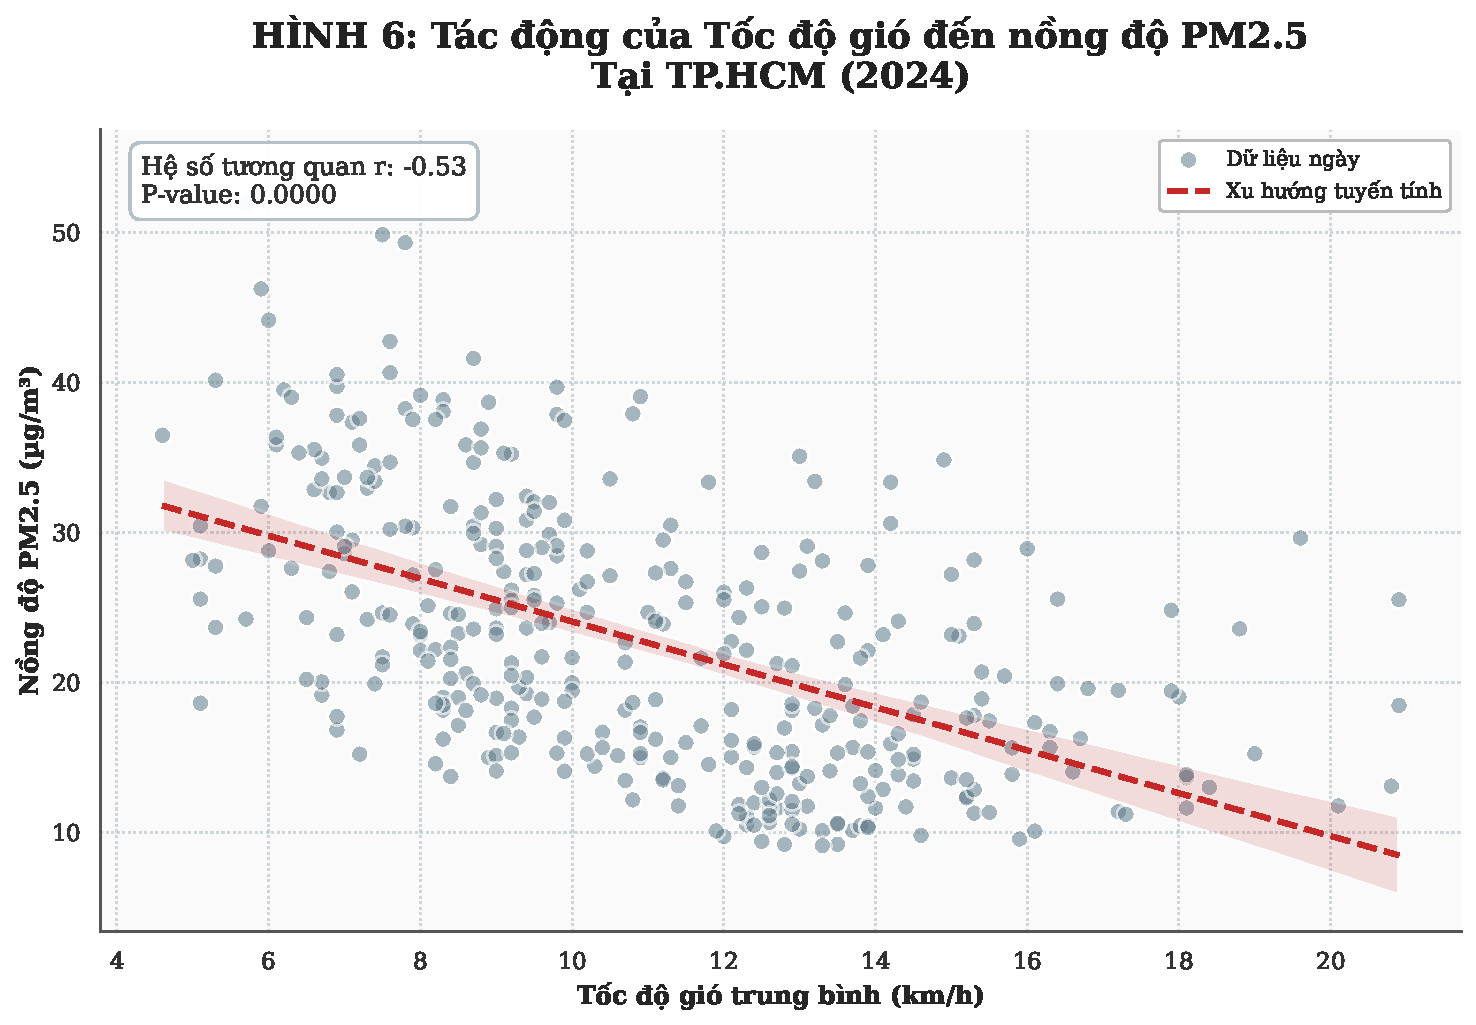
\includegraphics[width=0.95\textwidth]{../figures/06_wind_pm25_scatter.pdf}
\caption{Scatter plot thể hiện mối quan hệ giữa tốc độ gió và nồng độ \pmtwofive{}.}
\label{fig:wind-pm25}
\end{figure}

\textbf{Nhận xét:}
\begin{itemize}
    \item Xu hướng tương quan âm nhẹ: gió mạnh giúp giảm \pmtwofive{}
    \item Khi tốc độ gió $<$ 10 km/h, \pmtwofive{} có xu hướng cao và biến động lớn
    \item Gió $>$ 15 km/h giúp khuếch tán bụi hiệu quả, \pmtwofive{} thường $<$ 30 \ugm{}
\end{itemize}

\subsection{Mối quan hệ nhiệt độ và Ozone}

\begin{figure}[H]
\centering
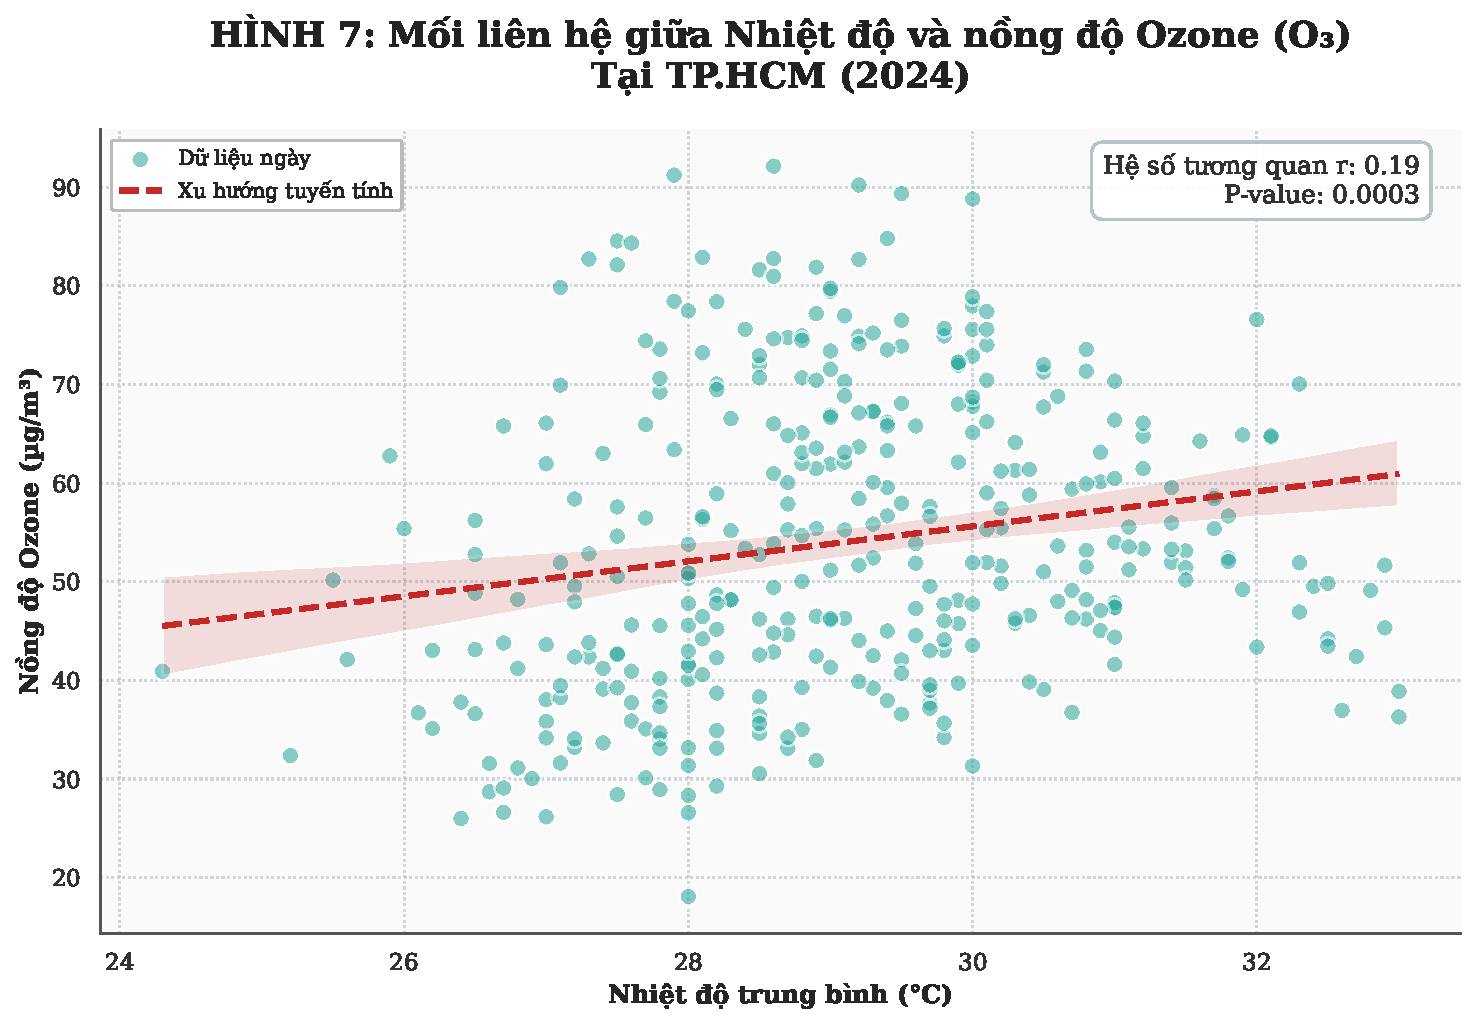
\includegraphics[width=0.95\textwidth]{../figures/7_temp_ozone_scatter.pdf}
\caption{Scatter plot cho thấy mối quan hệ dương giữa nhiệt độ và nồng độ \ozone{}.}
\label{fig:temp-ozone}
\end{figure}

\textbf{Nhận xét:}
\begin{itemize}
    \item Mối tương quan dương rõ rệt: nhiệt độ tăng làm tăng \ozone{}
    \item Nguyên nhân: phản ứng quang hóa tạo \ozone{} diễn ra mạnh hơn ở nhiệt độ cao
    \item Nhiệt độ $>$ 30\degreec{}: \ozone{} thường $>$ 60 \ugm{}
\end{itemize}

\subsection{So sánh PM2.5 và PM10}

\begin{figure}[H]
\centering
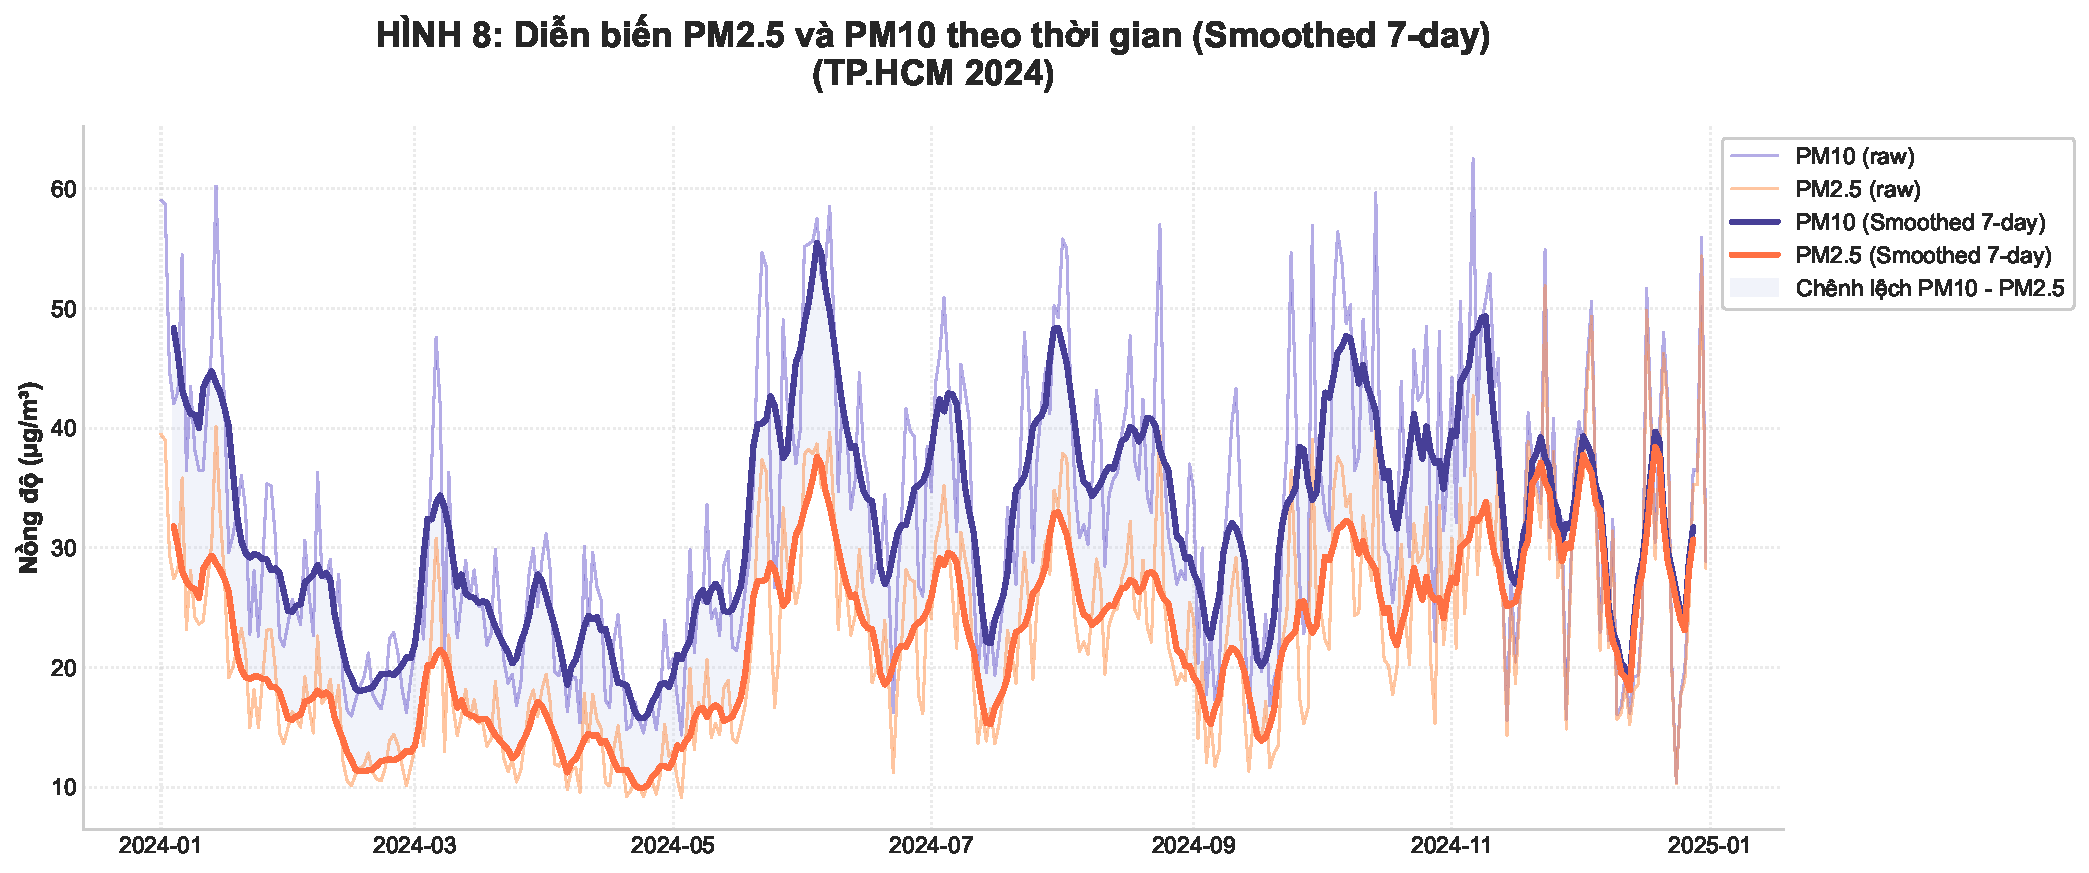
\includegraphics[width=0.95\textwidth]{../figures/8_pm25_vs_pm10_timeseries.pdf}
\caption{Time series so sánh xu hướng của \pmtwofive{} và \pmten{} qua thời gian.}
\label{fig:pm25-pm10}
\end{figure}

\textbf{Nhận xét:}
\begin{itemize}
    \item \pmten{} luôn cao hơn \pmtwofive{} (vì bao gồm cả \pmtwofive{})
    \item Xu hướng biến động tương đồng nhau (correlation cao)
    \item Tỷ lệ \pmtwofive{}/\pmten{} trung bình khoảng 0.7 (70\%)
\end{itemize}

\subsection{Phân loại AQI}

\begin{figure}[H]
\centering
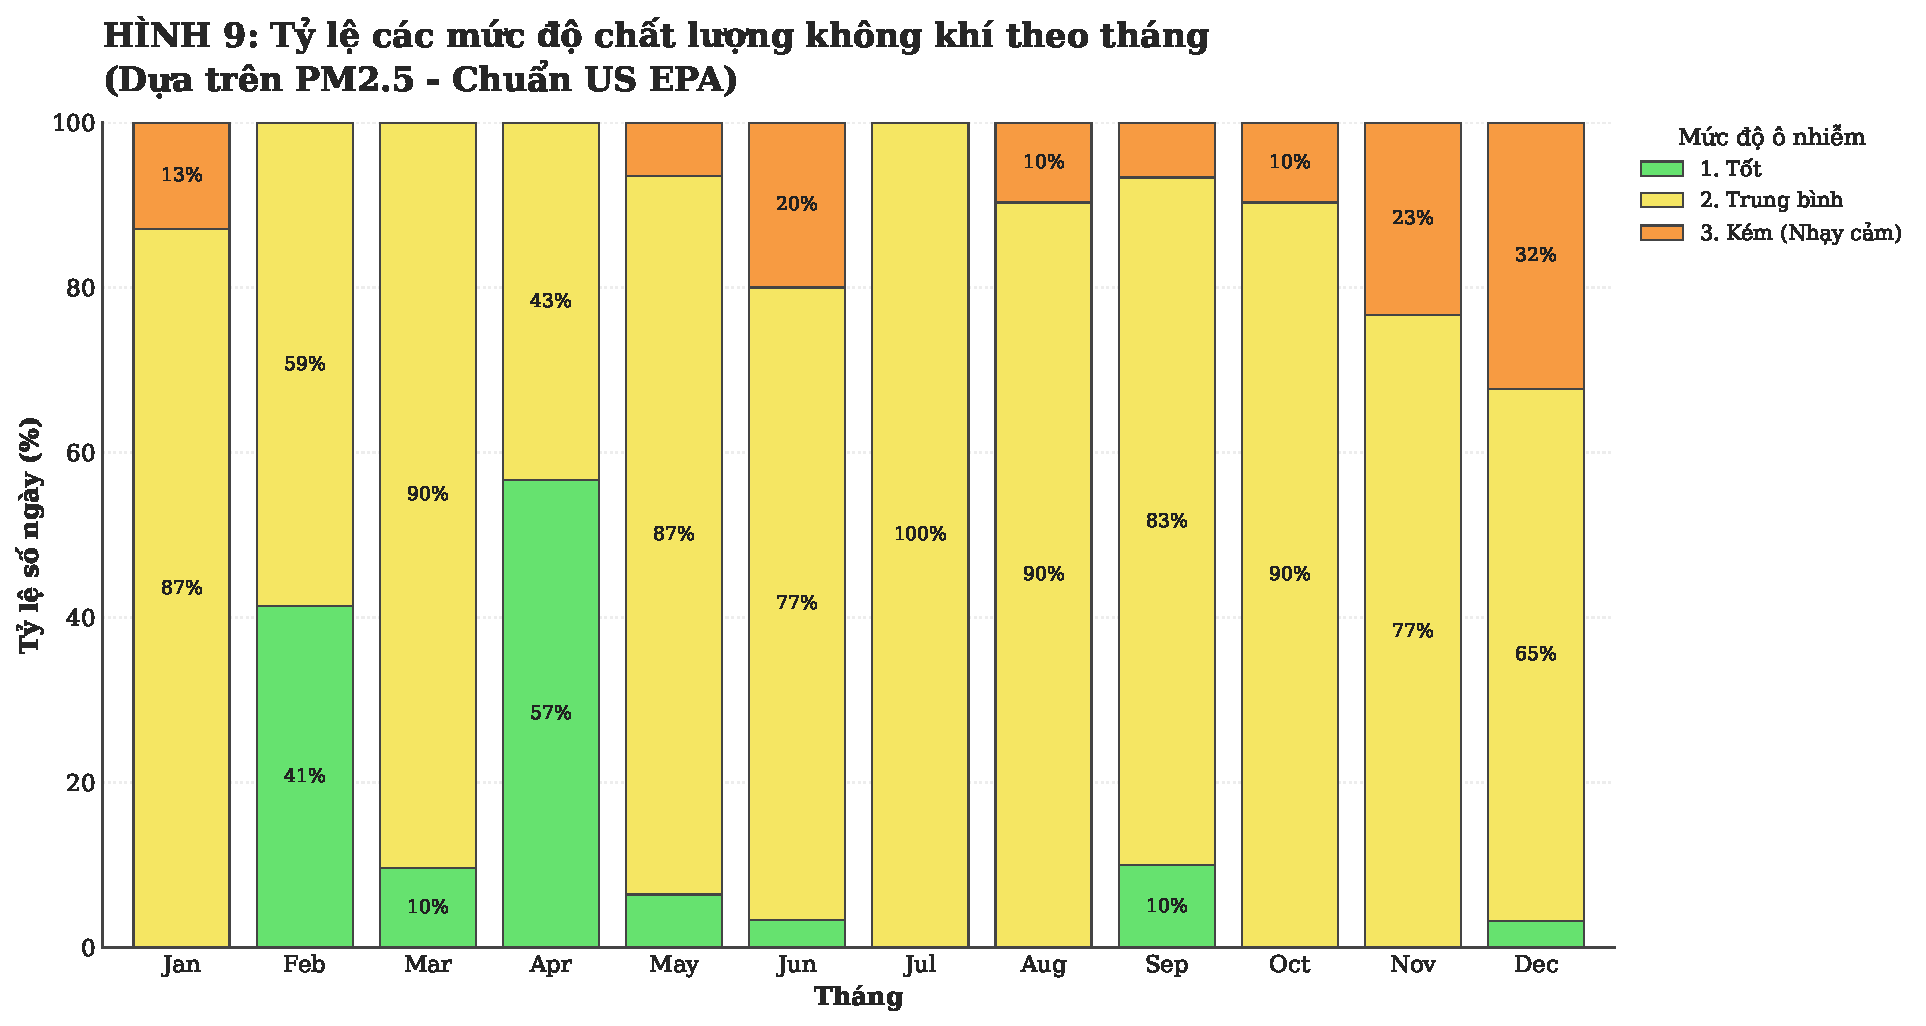
\includegraphics[width=0.95\textwidth]{../figures/09_aqi_category_stacked_bar.pdf}
\caption{Phân bố các category AQI theo tháng năm 2024.}
\label{fig:aqi-categories}
\end{figure}

\textbf{Nhận xét:}
\begin{itemize}
    \item Tháng 12, 1, 2: tỷ lệ "Unhealthy for Sensitive Groups" cao nhất
    \item Tháng 6, 7, 8: chủ yếu ở mức "Good" và "Moderate"
    \item Không có ngày nào đạt mức "Very Unhealthy" hoặc "Hazardous"
\end{itemize}

\section{Các phân tích nâng cao}

\subsection{Dự báo PM2.5 ngày tiếp theo}

\subsubsection{Mục tiêu}
Xây dựng mô hình dự báo nồng độ \pmtwofive{} cho \textbf{ngày tiếp theo} dựa trên dữ liệu lịch sử và điều kiện thời tiết hiện tại.

\subsubsection{Phương pháp}

\textbf{Model:} Linear Regression

\textbf{Features (15 biến):}
\begin{enumerate}
    \item \textbf{Lag features (3):} \pmtwofive{} của 1, 2, 3 ngày trước
    \item \textbf{Rolling averages (2):} Trung bình \pmtwofive{} trong 3 ngày, 7 ngày
    \item \textbf{Weather features (5):} Nhiệt độ, lượng mưa, tốc độ gió, áp suất, độ ẩm (của ngày hiện tại)
    \item \textbf{Air quality features (3):} \pmten{}, \ozone{}, CO (của ngày hiện tại)
    \item \textbf{Temporal features (2):} Ngày trong tuần, tháng
\end{enumerate}

\textbf{Train/Test split:}
\begin{itemize}
    \item Training set: 280 ngày (80\%)
    \item Test set: 70 ngày (20\%)
    \item Phương pháp: Sequential split (giữ nguyên thứ tự thời gian)
\end{itemize}

\subsubsection{Phân tích dữ liệu}

\begin{figure}[H]
\centering
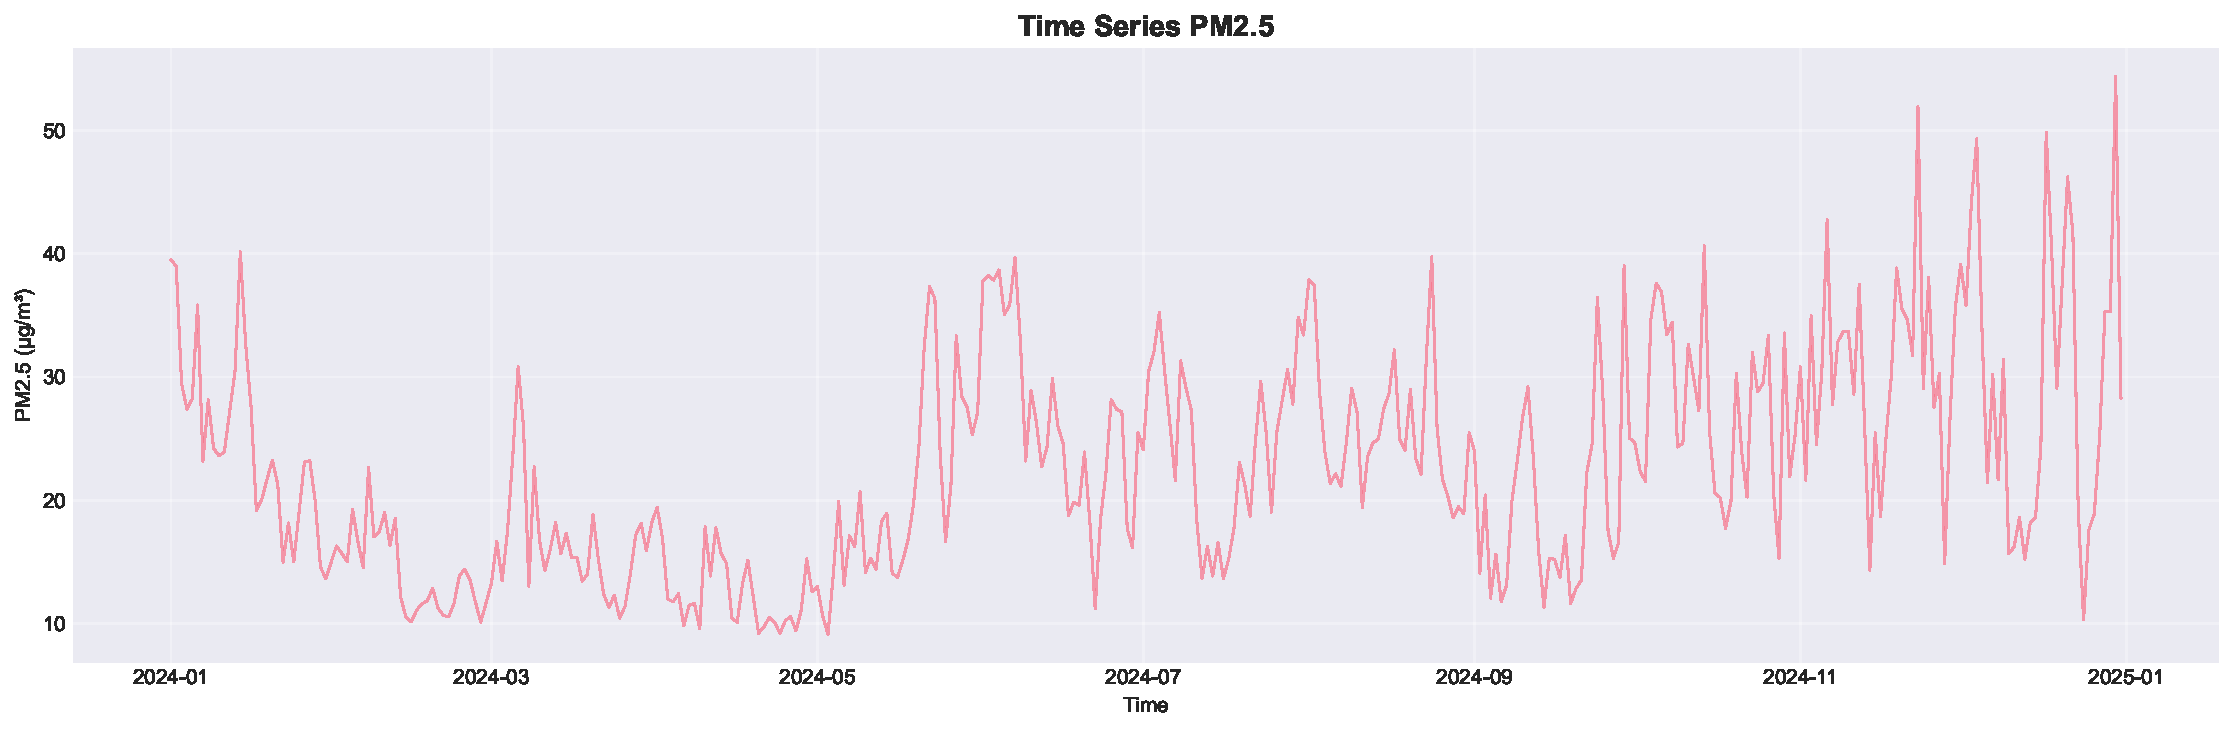
\includegraphics[width=0.95\textwidth]{../figures/14_timeseries_pm25.pdf}
\caption{Chuỗi thời gian \pmtwofive{} năm 2024 - dữ liệu đầu vào cho mô hình dự báo.}
\label{fig:timeseries-pm25-forecasting}
\end{figure}

\textbf{Nhận xét về dữ liệu:}
\begin{itemize}
    \item \pmtwofive{} có xu hướng theo mùa: tăng vào mùa khô (tháng 1-3, 11-12)
    \item Giảm vào mùa mưa (tháng 5-9)
    \item Dao động mạnh trong ngắn hạn - cần lag features và rolling averages
    \item Có xu hướng tự tương quan (autocorrelation) mạnh
\end{itemize}

\subsubsection{Kết quả dự báo}

\begin{figure}[H]
\centering
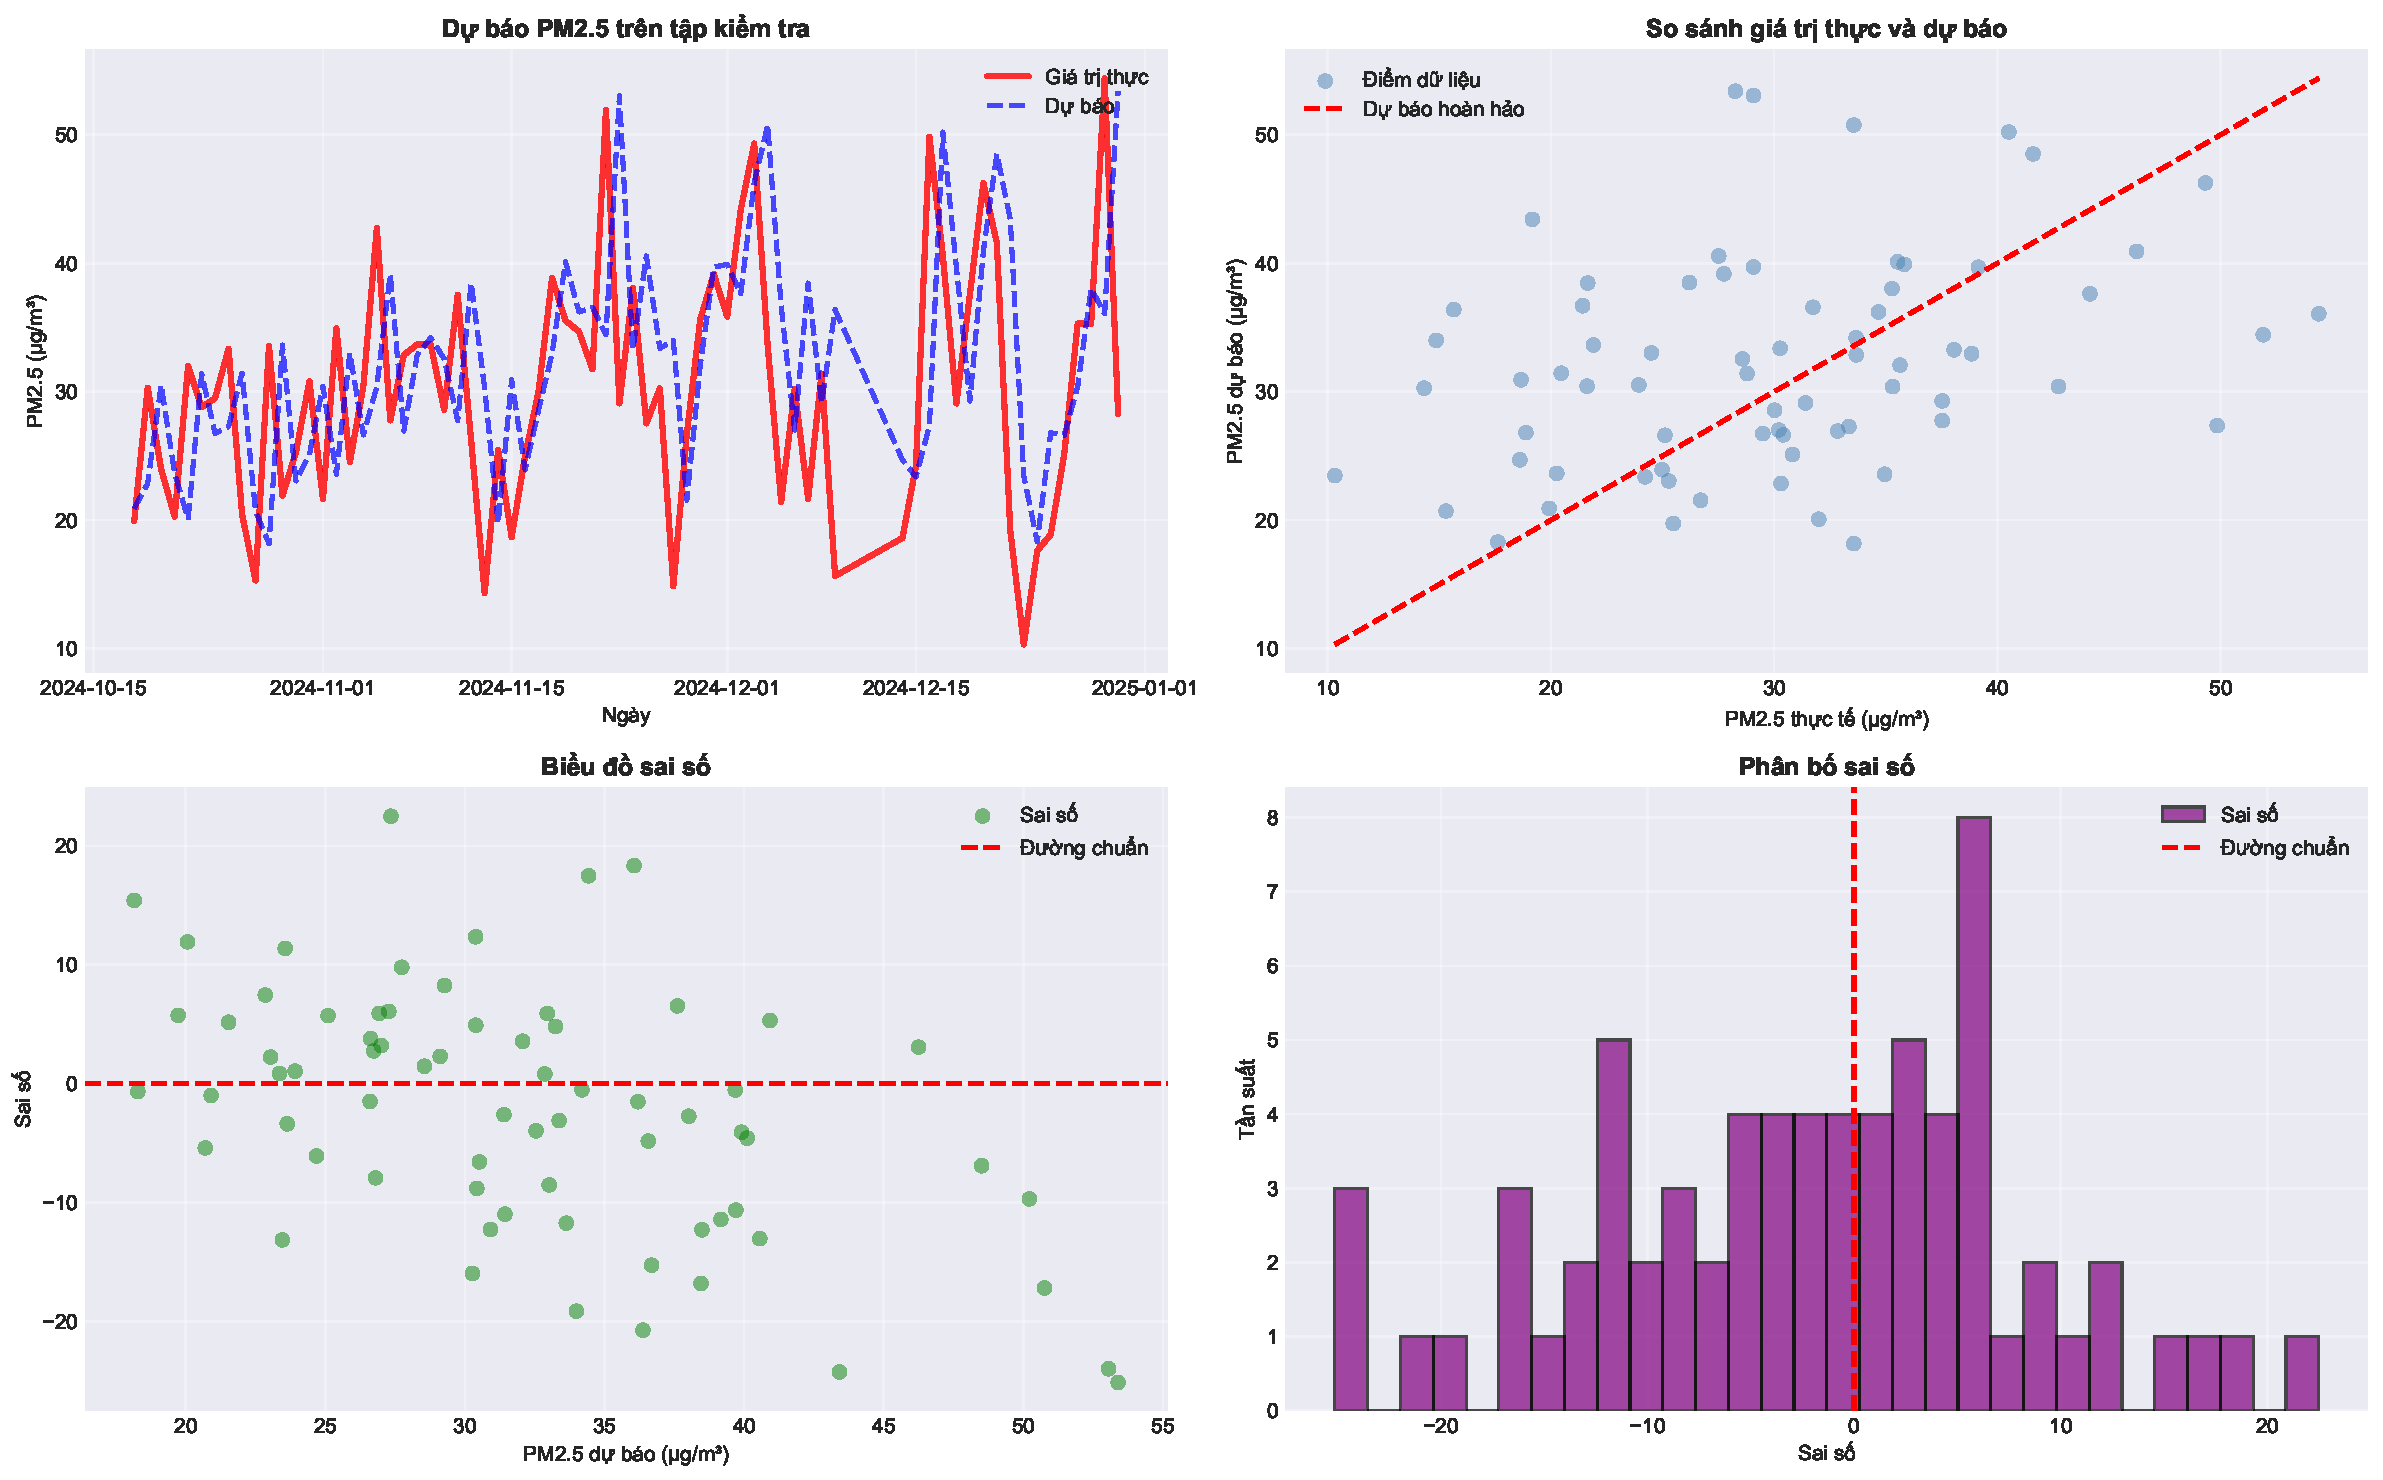
\includegraphics[width=0.95\textwidth]{../figures/13_pm25_predictions.pdf}
\caption{So sánh giá trị thực tế và dự báo \pmtwofive{} trên tập test. Scatter plot (trái) cho thấy mối tương quan; time series (phải) hiển thị dự báo theo thời gian.}
\label{fig:predictions-pm25}
\end{figure}

\begin{figure}[H]
\centering
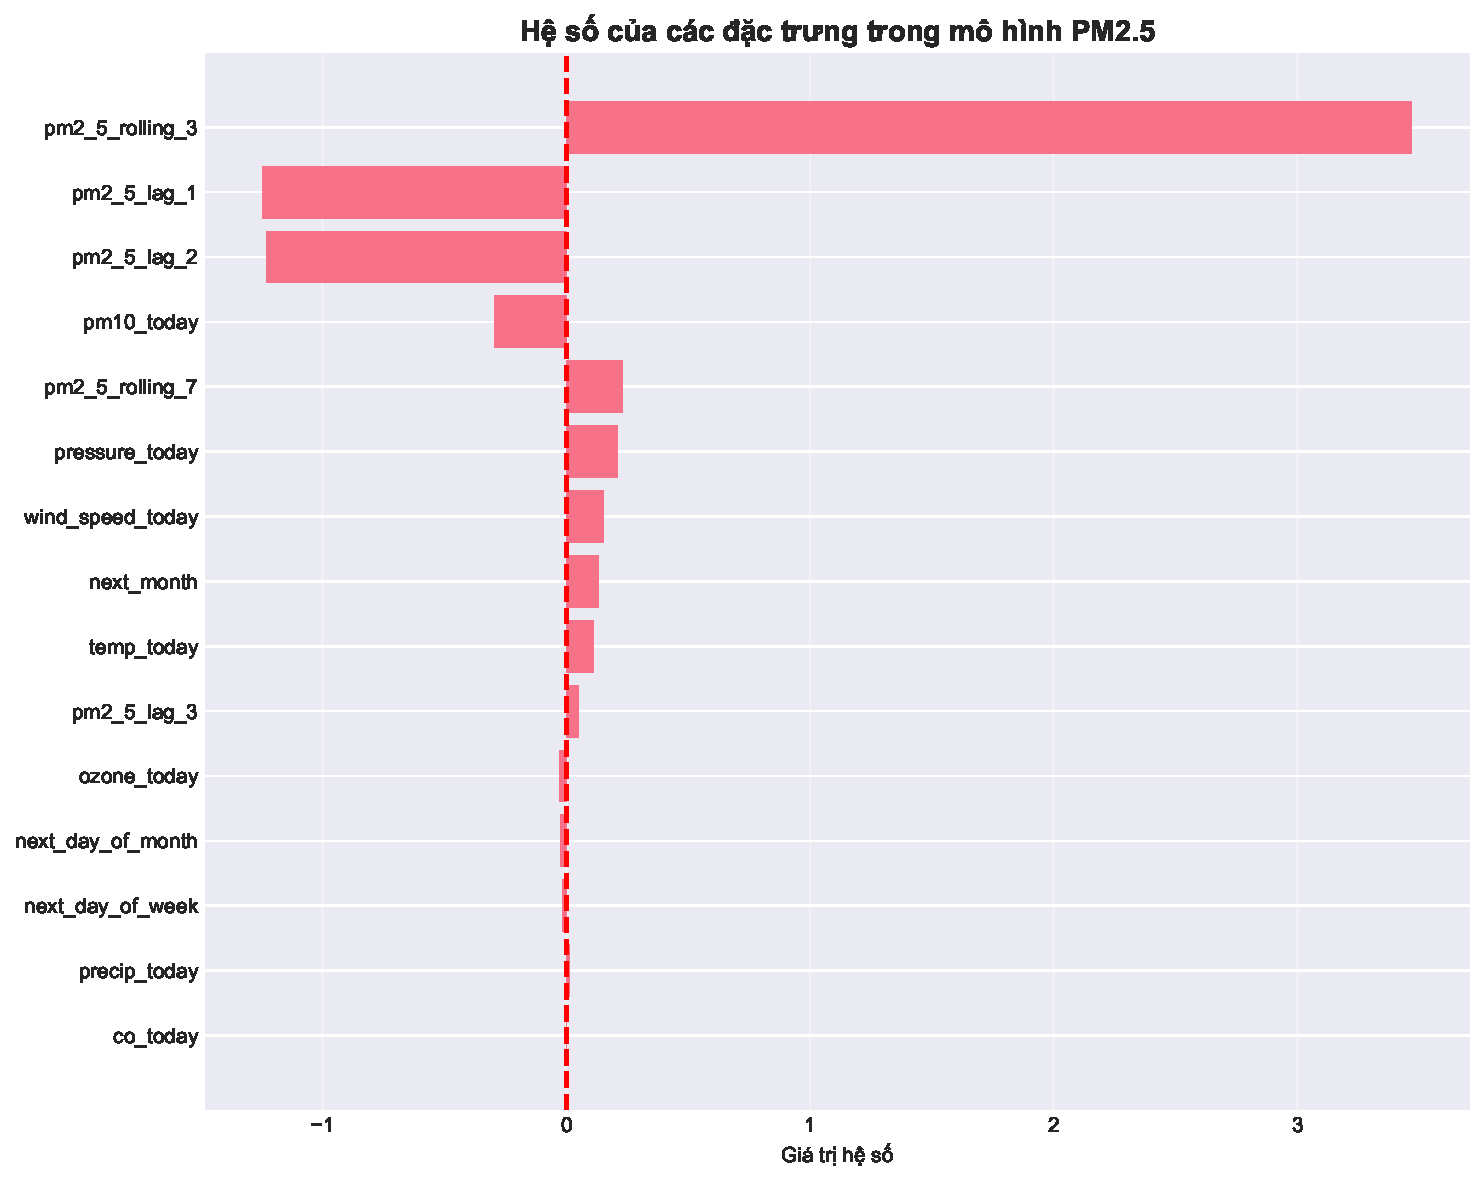
\includegraphics[width=0.95\textwidth]{../figures/12_feature_importance.pdf}
\caption{Top 10 features quan trọng nhất trong mô hình dự báo \pmtwofive{}. Các lag features và rolling averages có ảnh hưởng lớn nhất.}
\label{fig:feature-importance}
\end{figure}

\subsubsection{Đánh giá mô hình}

\begin{table}[H]
\centering
\caption{Kết quả dự báo PM2.5}
\label{tab:forecasting-results}
\begin{tabular}{lccccc}
\toprule
\textbf{Dataset} & \textbf{Size} & \textbf{MAE} & \textbf{MAPE} & \textbf{RMSE} & \textbf{R²} \\
\midrule
Training & 280 & 3.41 & 16.84\% & 4.50 & 0.675 \\
Test & 70 & 8.36 & 32.71\% & 10.56 & -0.284 \\
\bottomrule
\end{tabular}
\end{table}

\textbf{Giải thích metrics:}
\begin{itemize}
    \item \textbf{MAE (Mean Absolute Error):} Sai số trung bình tuyệt đối (\ugm{})
    \begin{equation}
    \text{MAE} = \frac{1}{n}\sum_{i=1}^{n}|y_i - \hat{y}_i|
    \end{equation}
    
    \item \textbf{MAPE (Mean Absolute Percentage Error):} Sai số phần trăm trung bình (\%)
    \begin{equation}
    \text{MAPE} = \frac{100\%}{n}\sum_{i=1}^{n}\left|\frac{y_i - \hat{y}_i}{y_i}\right|
    \end{equation}
    
    \item \textbf{RMSE (Root Mean Squared Error):} Căn bậc hai của sai số bình phương trung bình (\ugm{})
    \begin{equation}
    \text{RMSE} = \sqrt{\frac{1}{n}\sum_{i=1}^{n}(y_i - \hat{y}_i)^2}
    \end{equation}
    
    \item \textbf{R² (Coefficient of Determination):} Hệ số xác định (0-1, càng cao càng tốt)
    \begin{equation}
    R^2 = 1 - \frac{\sum_{i=1}^{n}(y_i - \hat{y}_i)^2}{\sum_{i=1}^{n}(y_i - \bar{y})^2}
    \end{equation}
\end{itemize}

\subsubsection{Diễn giải kết quả}

\textbf{Hiệu suất trên Training set:}
\begin{itemize}
    \item MAE = 3.41 \ugm{}: Mô hình dự báo sai trung bình 3.41 \ugm{}
    \item MAPE = 16.84\%: Sai số tương đối khoảng 17\%
    \item R² = 0.675: Mô hình giải thích được 67.5\% phương sai của \pmtwofive{}
\end{itemize}

\textbf{Hiệu suất trên Test set:}
\begin{itemize}
    \item MAE = 8.36 \ugm{}: Sai số tăng gấp 2.5 lần so với training
    \item MAPE = 32.71\%: Sai số tương đối tăng lên 33\%
    \item R² = -0.284: Mô hình kém hơn việc dự báo bằng giá trị trung bình
\end{itemize}

\textbf{Nguyên nhân overfitting:}
\begin{itemize}
    \item Chênh lệch lớn giữa training và test performance
    \item Model quá đơn giản (Linear Regression) không capture được non-linear patterns
    \item \pmtwofive{} chịu ảnh hưởng nhiều yếu tố ngoại sinh khó dự đoán
    \item Cần thử các model phức tạp hơn: Random Forest, XGBoost, LSTM
\end{itemize}

\subsection{Phân cụm điều kiện môi trường (K-Means Clustering)}

\subsubsection{Mục tiêu}
Nhóm các ngày có điều kiện môi trường tương tự nhau để phát hiện patterns và đặc điểm của từng nhóm.

\subsubsection{Phương pháp}
\begin{itemize}
    \item \textbf{Algorithm:} K-Means Clustering
    \item \textbf{Số cụm (K):} 4 clusters
    \item \textbf{Features:} Nhiệt độ, lượng mưa, tốc độ gió, UV Index, \pmtwofive{}, \ozone{}
    \item \textbf{Preprocessing:} StandardScaler normalization
\end{itemize}

\subsubsection{Kết quả phân cụm}

\begin{table}[H]
\centering
\caption{Đặc điểm các cụm điều kiện môi trường}
\label{tab:clustering}
\small
\begin{tabular}{lcccccccc}
\toprule
\textbf{Cụm} & \textbf{Ngày} & \textbf{Tỷ tr.} & \textbf{Temp} & \textbf{Precip} & \textbf{Wind} & \textbf{UV} & \textbf{PM2.5} & \textbf{O3} \\
 & & \textbf{(\%)} & \textbf{(\degreec{})} & \textbf{(mm)} & \textbf{(km/h)} & & \textbf{(\ugm{})} & \textbf{(\ugm{})} \\
\midrule
Mưa & 59 & 16.7 & 28.06 & 16.63 & 13.84 & 7.59 & 20.62 & 41.03 \\
Mưa-Bụi cao & 94 & 26.6 & 28.17 & 5.98 & 8.19 & 7.31 & 30.47 & 45.46 \\
Nóng-Sạch & 119 & 33.6 & 30.69 & 1.38 & 13.09 & 10.78 & 15.99 & 56.71 \\
Trung tính & 82 & 23.2 & 28.86 & 1.17 & 8.97 & 8.79 & 25.54 & 72.03 \\
\bottomrule
\end{tabular}
\end{table}

\textbf{Đặc điểm từng cụm:}
\begin{enumerate}
    \item \textbf{Cụm "Mưa" (59 ngày, 16.7\%):} Lượng mưa cao nhất (16.63 mm/ngày), \pmtwofive{} trung bình (20.62 \ugm{}), UV thấp do mây che
    
    \item \textbf{Cụm "Mưa - Bụi cao" (94 ngày, 26.6\%):} \pmtwofive{} cao nhất (30.47 \ugm{}), mưa vừa phải nhưng không đủ để giảm bụi, tốc độ gió thấp (8.19 km/h)
    
    \item \textbf{Cụm "Nóng - Sạch" (119 ngày, 33.6\%):} Nhiệt độ cao nhất (30.69 \degreec{}), \pmtwofive{} thấp nhất (15.99 \ugm{}), UV cao, gió mạnh
    
    \item \textbf{Cụm "Trung tính/Giao mùa" (82 ngày, 23.2\%):} Các chỉ số ở mức trung bình, \ozone{} cao nhất (72.03 \ugm{})
\end{enumerate}

\subsubsection{Trực quan hóa phân cụm}

\begin{figure}[H]
\centering
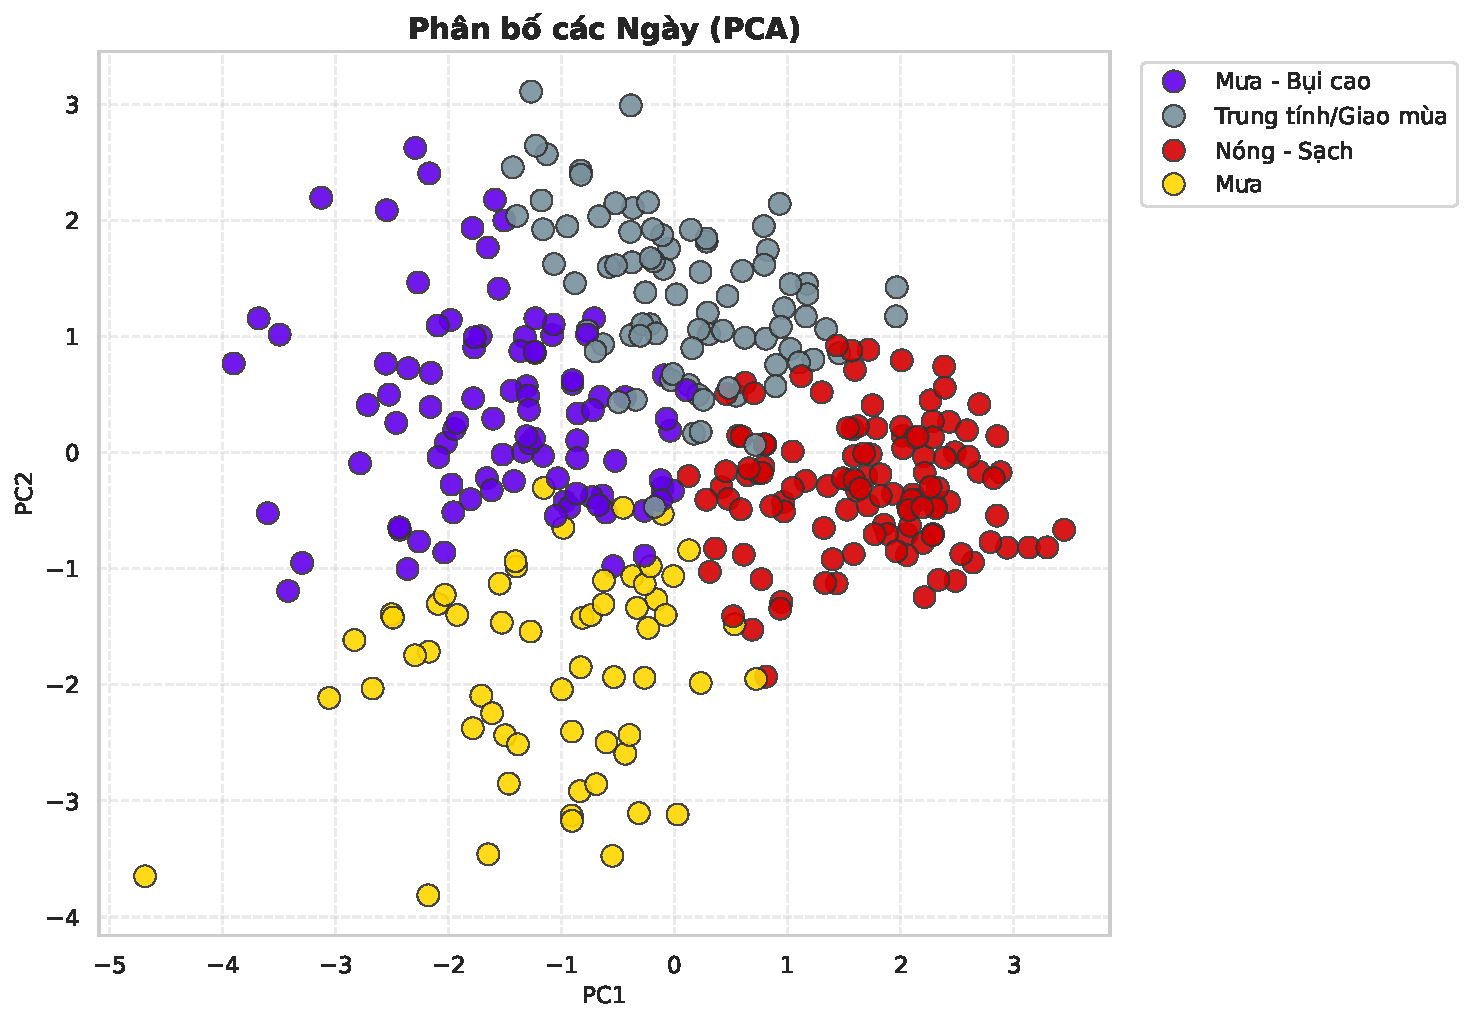
\includegraphics[width=0.95\textwidth]{../figures/10_kmeans_pca_scatter_yellow_rain.pdf}
\caption{Biểu đồ PCA scatter plot của 4 cụm điều kiện môi trường.}
\label{fig:kmeans-pca}
\end{figure}

\begin{figure}[H]
\centering
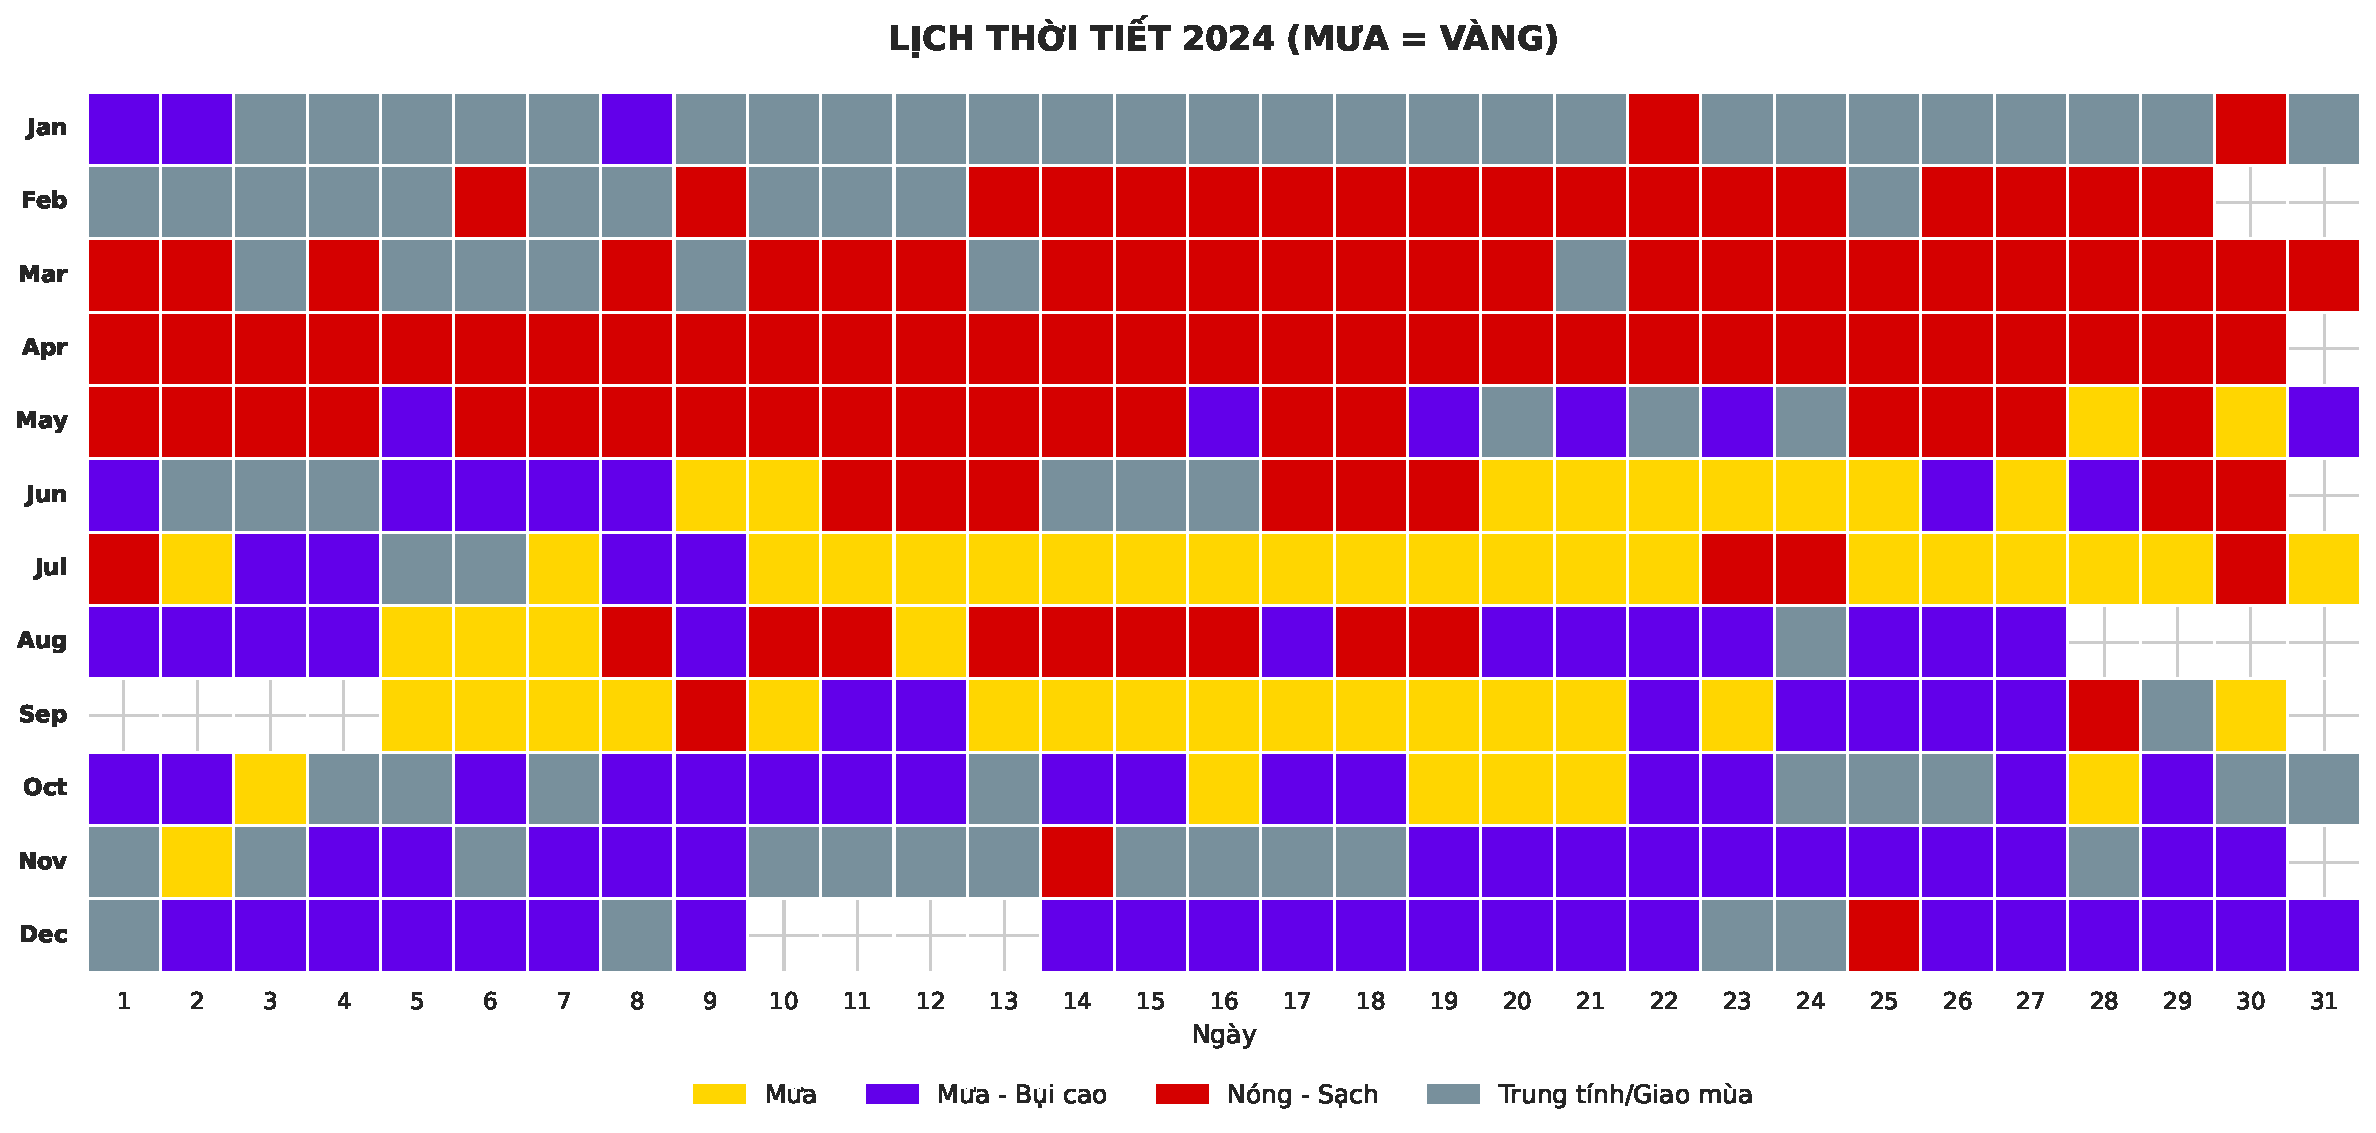
\includegraphics[width=0.95\textwidth]{../figures/11_kmeans_calendar_heatmap_yellow.pdf}
\caption{Calendar heatmap hiển thị phân bố các cụm theo ngày trong năm 2024.}
\label{fig:kmeans-calendar}
\end{figure}

\textbf{Nhận xét từ calendar heatmap:}
\begin{itemize}
    \item Cụm "Nóng - Sạch" (xanh lá) phổ biến nhất, xuất hiện nhiều vào mùa hè
    \item Cụm "Mưa - Bụi cao" (vàng) tập trung vào đầu và cuối năm
    \item Cụm "Mưa" (xanh dương) xuất hiện chủ yếu trong mùa mưa (tháng 5-10)
    \item Phân bố cụm có tính thời vụ rõ rệt
\end{itemize}

\subsection{Phát hiện bất thường (Anomaly Detection)}

\subsubsection{Phương pháp}

Sử dụng \textbf{Isolation Forest} để phát hiện các ngày có chất lượng không khí bất thường:
\begin{itemize}
    \item \textbf{Algorithm:} Isolation Forest
    \item \textbf{Contamination:} 10\% (giả định 10\% ngày là anomalies)
    \item \textbf{Features:} \pmtwofive{}, \pmten{}, lượng mưa, tốc độ gió, nhiệt độ
\end{itemize}

\subsubsection{Các ngày Case Study}

Hai ngày được chọn để phân tích chi tiết:

\begin{figure}[H]
\centering
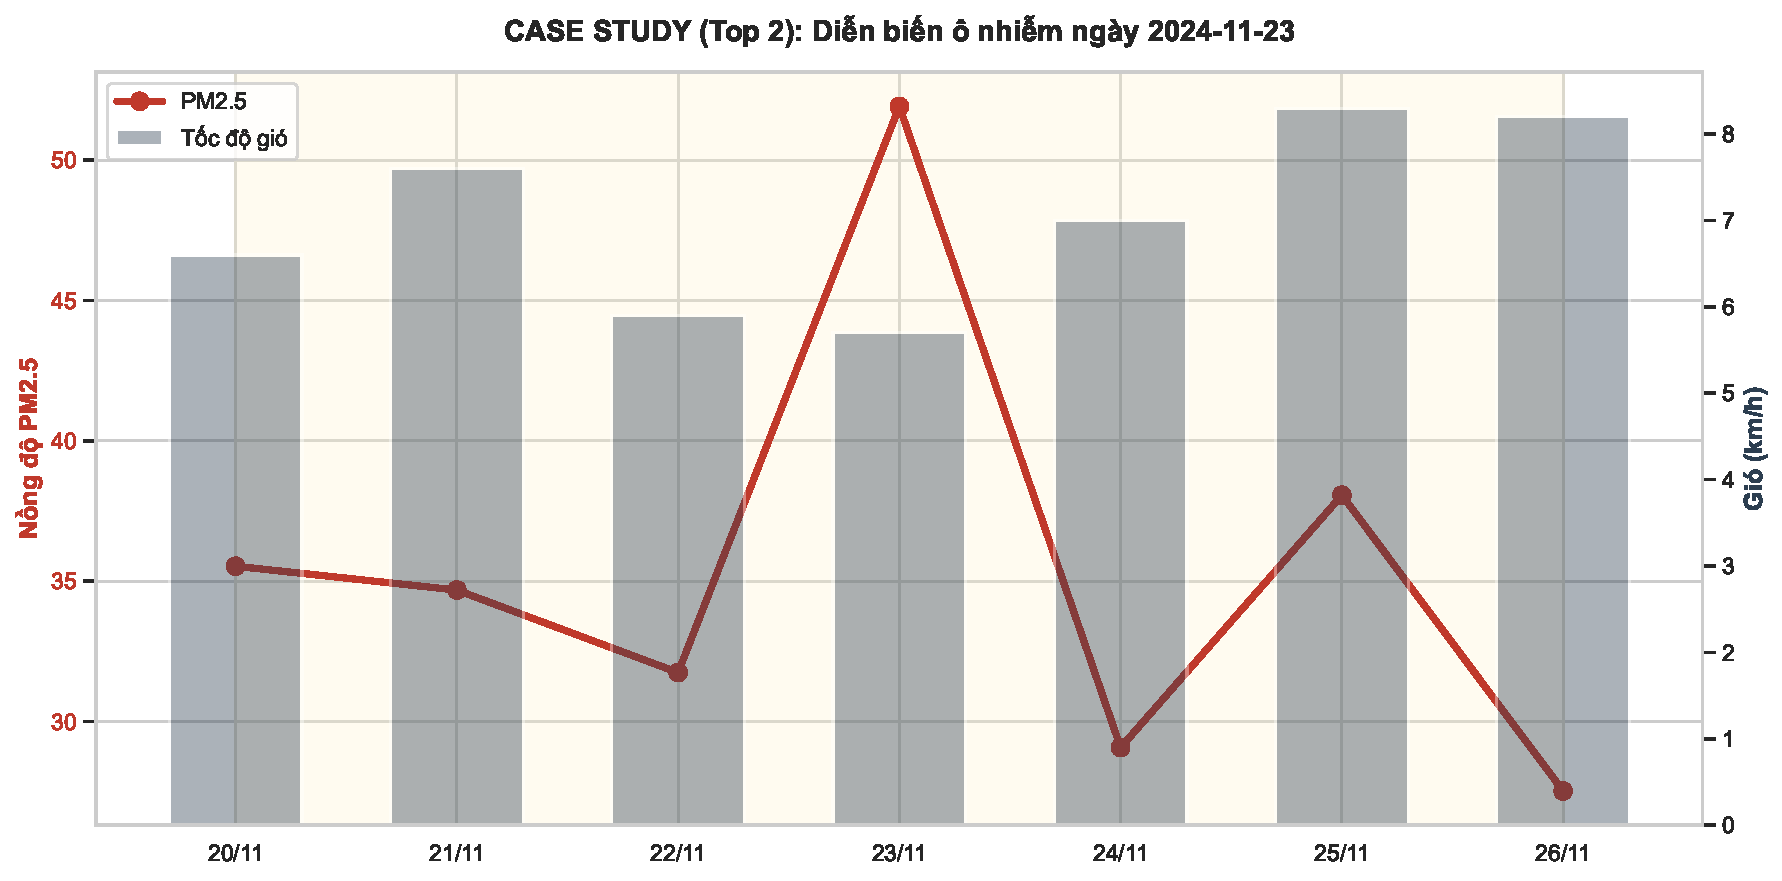
\includegraphics[width=0.95\textwidth]{../figures/case_study_rank2_2024-11-23.pdf}
\caption{Case Study Top 2: Diễn biến ô nhiễm ngày 23/11/2024 - một trong những ngày có PM2.5 cao nhất.}
\label{fig:case-study-rank2}
\end{figure}

\textbf{Ngày 23/11/2024 - Top 2 ngày ô nhiễm cao nhất:}
\begin{itemize}
    \item \pmtwofive{}: 52.8 \ugm{} (vượt ngưỡng EPA 35 \ugm{})
    \item Tốc độ gió yếu: 7.2 km/h
    \item Lượng mưa: 0 mm (thời tiết khô hanh)
    \item Xu hướng: Tăng dần từ ngày 20/11, đỉnh điểm 23/11, sau đó giảm
\end{itemize}

\begin{figure}[H]
\centering
\includegraphics[width=0.95\textwidth]{../figures/case_study_zoom_2024-12-30.pdf}
\caption{Case Study ngày tệ nhất: Phân tích chi tiết sự kiện ô nhiễm nặng ngày 30/12/2024.}
\label{fig:case-study-worst}
\end{figure}

\textbf{Ngày 30/12/2024 - Ngày ô nhiễm tệ nhất:}
\begin{itemize}
    \item \pmtwofive{}: 56.9 \ugm{} (cao nhất cả năm)
    \item AQI Category: Unhealthy for Sensitive Groups
    \item Điều kiện thời tiết: Không mưa, gió yếu, nhiệt độ cao
    \item Xu hướng: Tích tụ dần trong nhiều ngày liên tiếp
\end{itemize}

\textbf{Nhận xét chung về các ngày bất thường:}
\begin{itemize}
    \item Thường xảy ra vào cuối năm (tháng 11-12) - mùa khô
    \item Kết hợp giữa gió yếu ($<$ 10 km/h) và không mưa
    \item \pmtwofive{} tăng dần trong 3-5 ngày, sau đó giảm khi có gió hoặc mưa
    \item Cần cảnh báo sớm khi xuất hiện dấu hiệu: gió yếu + khô hanh kéo dài
\end{itemize}

\section{Diễn giải và Kết luận}

\subsection{Phát hiện chính}

\begin{enumerate}
    \item \textbf{Chất lượng không khí TP.HCM năm 2024:}
    \begin{itemize}
        \item \pmtwofive{} trung bình: 22.67 \ugm{} (cao hơn ngưỡng WHO: 15 \ugm{})
        \item 63.9\% số ngày vượt ngưỡng WHO, 36.1\% vượt ngưỡng US EPA
        \item Chất lượng không khí chưa đạt tiêu chuẩn quốc tế
    \end{itemize}
    
    \item \textbf{Xu hướng theo mùa:}
    \begin{itemize}
        \item \pmtwofive{} cao vào mùa khô (tháng 1-3, 11-12)
        \item \pmtwofive{} thấp vào mùa mưa (tháng 5-9)
        \item Lượng mưa có tác động tích cực đến chất lượng không khí
    \end{itemize}
    
    \item \textbf{Mối quan hệ thời tiết - chất lượng không khí:}
    \begin{itemize}
        \item Mưa giúp giảm \pmtwofive{}, nhưng cần lượng mưa đủ lớn
        \item Gió mạnh giúp khuếch tán bụi hiệu quả
        \item Nhiệt độ cao kết hợp với gió mạnh tạo điều kiện tốt cho không khí sạch
    \end{itemize}
    
    \item \textbf{Phân cụm môi trường:}
    \begin{itemize}
        \item Xác định được 4 loại điều kiện môi trường đặc trưng
        \item Cụm "Nóng - Sạch" chiếm tỷ trọng lớn nhất (33.6\%)
        \item Cụm "Mưa - Bụi cao" là trường hợp đáng chú ý (26.6\%)
    \end{itemize}
    
    \item \textbf{Khả năng dự báo PM2.5:}
    \begin{itemize}
        \item Linear Regression cho kết quả chấp nhận được trên training set
        \item Overfitting trên test set cho thấy cần model phức tạp hơn
        \item Lag features và rolling averages là predictors quan trọng nhất
    \end{itemize}
\end{enumerate}

\subsection{Bối cảnh và ý nghĩa}

Kết quả phân tích cho thấy chất lượng không khí TP.HCM năm 2024 chưa đạt tiêu chuẩn của WHO, với hơn 60\% số ngày có \pmtwofive{} vượt ngưỡng an toàn. Điều này đặt ra thách thức cho sức khỏe cộng đồng, đặc biệt là nhóm nhạy cảm (trẻ em, người cao tuổi, người có bệnh hô hấp).

Mối quan hệ giữa thời tiết và chất lượng không khí được xác nhận rõ ràng: mùa mưa giúp cải thiện chất lượng không khí đáng kể, trong khi mùa khô có xu hướng tích tụ bụi. Phát hiện này có thể hỗ trợ hoạch định chính sách quản lý chất lượng không khí theo mùa.

Phân cụm K-Means đã giúp nhận diện 4 loại điều kiện môi trường đặc trưng, trong đó cụm "Mưa - Bụi cao" cần được quan tâm đặc biệt vì kết hợp giữa điều kiện thời tiết không thuận lợi và ô nhiễm cao.

\subsection{Giới hạn của nghiên cứu}

\begin{enumerate}
    \item \textbf{Dữ liệu:}
    \begin{itemize}
        \item Chỉ có dữ liệu của 1 năm (2024), chưa đủ để phân tích xu hướng dài hạn
        \item Thiếu một số biến quan trọng (hướng gió, \cotwo{})
        \item Dữ liệu tại 1 điểm, chưa đại diện cho toàn TP.HCM
    \end{itemize}
    
    \item \textbf{Mô hình dự báo:}
    \begin{itemize}
        \item Linear Regression quá đơn giản, không capture được non-linear patterns
        \item Overfitting trên test set
        \item Chưa xem xét yếu tố ngoại sinh (giao thông, công nghiệp, cháy rừng)
    \end{itemize}
    
    \item \textbf{Phương pháp:}
    \begin{itemize}
        \item Chưa áp dụng kỹ thuật feature selection
        \item Chưa thử các thuật toán advanced (ensemble methods, deep learning)
        \item Chưa có cross-validation để đánh giá robustness
    \end{itemize}
\end{enumerate}

\subsection{Đề xuất tiếp theo}

\begin{enumerate}
    \item \textbf{Mở rộng dữ liệu:}
    \begin{itemize}
        \item Thu thập dữ liệu nhiều năm để phân tích xu hướng dài hạn
        \item Thêm nhiều điểm đo tại các quận/huyện khác nhau
        \item Tích hợp dữ liệu về giao thông, hoạt động công nghiệp
    \end{itemize}
    
    \item \textbf{Cải thiện mô hình dự báo:}
    \begin{itemize}
        \item Thử các model phức tạp: Random Forest, XGBoost, LSTM
        \item Áp dụng feature engineering nâng cao
        \item Implement ensemble methods để kết hợp nhiều models
    \end{itemize}
    
    \item \textbf{Phân tích sâu hơn:}
    \begin{itemize}
        \item Phân tích tác động của các sự kiện đặc biệt (lễ, tết, lockdown)
        \item Nghiên cứu correlation giữa \pmtwofive{} và các chỉ số sức khỏe cộng đồng
        \item Xây dựng hệ thống cảnh báo sớm cho ngày có chất lượng không khí xấu
    \end{itemize}
    
    \item \textbf{Ứng dụng thực tế:}
    \begin{itemize}
        \item Xây dựng dashboard real-time monitoring
        \item Tích hợp với hệ thống dự báo thời tiết để tư vấn cho người dân
        \item Hỗ trợ hoạch định chính sách quản lý chất lượng không khí
    \end{itemize}
\end{enumerate}

\section{Tài liệu tham khảo}

\subsection{Nguồn dữ liệu}
\begin{enumerate}
    \item Meteostat - Weather and Climate Data. \url{https://meteostat.net}
    \item Open-Meteo Air Quality API. \url{https://open-meteo.com/en/docs/air-quality-api}
\end{enumerate}

\subsection{Tiêu chuẩn và phương pháp}
\begin{enumerate}
    \item World Health Organization (WHO). WHO Global Air Quality Guidelines, 2021.
    \item U.S. Environmental Protection Agency (EPA). Air Quality Index (AQI) Technical Assistance Document.
    \item U.S. EPA. AirNow.gov - Air Quality Index Calculator. \url{https://www.airnow.gov/aqi/aqi-calculator/}
\end{enumerate}

\subsection{Thư viện Python}
\begin{enumerate}
    \item Pandas (v2.x) - Data manipulation and analysis. \url{https://pandas.pydata.org}
    \item NumPy (v1.x) - Numerical computing. \url{https://numpy.org}
    \item Matplotlib (v3.x) - Data visualization. \url{https://matplotlib.org}
    \item Seaborn (v0.x) - Statistical data visualization. \url{https://seaborn.pydata.org}
    \item Scikit-learn (v1.x) - Machine learning. \url{https://scikit-learn.org}
    \item Meteostat Python Library. \url{https://dev.meteostat.net/python/}
\end{enumerate}

\subsection{Phương pháp máy học}
\begin{enumerate}
    \item Pedregosa et al. (2011). Scikit-learn: Machine Learning in Python. JMLR 12, pp. 2825-2830.
    \item Hastie, T., Tibshirani, R., \& Friedman, J. (2009). The Elements of Statistical Learning: Data Mining, Inference, and Prediction. Springer.
\end{enumerate}

\appendix
\section{Cấu trúc thư mục dự án}

\begin{verbatim}
2526-LTXLDL-PROJECT-AIT2006-2-3.4/
|-- raw/                          # Du lieu goc
|   |-- meteostat_weather_data.csv
|   +-- open-meteo-hourly-AQ.csv
|
|-- processed/                    # Du lieu da xu ly
|   |-- weather_cleaned.csv
|   |-- airquality_cleaned.csv
|   |-- final_combined_data.csv
|   +-- [aggregated files...]
|
|-- reports/                      # Bao cao va ket qua
|   |-- qa_weather_summary.csv
|   |-- qa_airquality_summary.csv
|   |-- statistics_summary.csv
|   +-- pm25_forecasting_results.csv
|
|-- figures/                      # Hinh anh (16 figures)
|   |-- 01_time_series.pdf
|   |-- 02_uv_index.pdf
|   |-- 03_Pm25_distribution.pdf
|   |-- 04_monthly_boxplot.pdf
|   |-- 05_correlation_matrix.pdf
|   |-- 06_wind_pm25_scatter.pdf
|   |-- 07_temp_ozone_scatter.pdf
|   |-- 08_pm25_vs_pm10_timeseries.pdf
|   |-- 09_aqi_category_stacked_bar.pdf
|   |-- 10_kmeans_pca_scatter.pdf
|   |-- 11_kmeans_calendar_heatmap.pdf
|   |-- 12_feature_importance.pdf
|   |-- 13_pm25_predictions.pdf
|   |-- 14_timeseries_pm25.pdf
|   |-- 15_case_study_rank2.pdf
|   +-- 16_case_study_zoom.pdf
|
+-- src/                          # Ma nguon
    |-- 01_weather_data_cleaning.ipynb
    |-- 02_airquality_data_cleaning.ipynb
    |-- 03_merge_and_sync.ipynb
    |-- 04_statistics_and_aggregation.ipynb
    |-- 05_visualization.ipynb
    |-- 06_pm25_forecasting.ipynb
    |-- 07_advanced_analysis.ipynb
    +-- 08_kmeans_clustering.ipynb
\end{verbatim}

\section{Danh sách hình ảnh}

\begin{table}[H]
\centering
\caption{Danh sách 16 figures được sử dụng trong báo cáo}
\begin{tabular}{clp{8cm}}
\toprule
\textbf{STT} & \textbf{Tên file} & \textbf{Mô tả} \\
\midrule
1 & 01\_time\_series.pdf & Meteogram tổng hợp \\
2 & 02\_uv\_index.pdf & UV Index theo thời gian \\
3 & 03\_Pm25\_distribution.pdf & Phân bố PM2.5 \\
4 & 04\_monthly\_boxplot.pdf & Boxplot theo tháng \\
5 & 05\_correlation\_matrix.pdf & Ma trận tương quan \\
6 & 06\_wind\_pm25\_scatter.pdf & Scatter gió vs PM2.5 \\
7 & 07\_temp\_ozone\_scatter.pdf & Scatter nhiệt độ vs O3 \\
8 & 08\_pm25\_vs\_pm10\_timeseries.pdf & So sánh PM2.5 và PM10 \\
9 & 09\_aqi\_category\_stacked\_bar.pdf & Phân loại AQI \\
10 & 10\_kmeans\_pca\_scatter.pdf & PCA scatter clustering \\
11 & 11\_kmeans\_calendar\_heatmap.pdf & Calendar heatmap \\
12 & 12\_feature\_importance.pdf & Feature importance \\
13 & 13\_pm25\_predictions.pdf & Kết quả dự báo \\
14 & 14\_timeseries\_pm25.pdf & Time series PM2.5 \\
15 & 15\_case\_study\_rank2.pdf & Case study rank 2 \\
16 & 16\_case\_study\_zoom.pdf & Case study ngày tệ nhất \\
\bottomrule
\end{tabular}
\end{table}

\end{document}
